\chapter{Implementation} \label{Chapter5}
In this chapter, the implementation of the various components of the research environment are described in-depth. This includes the challenges that were encountered in the implementation as well as alterations that were made to the system design as issues were unearthed.

In the interest of succinctness, low-level details of installation of tools etc. are not explained in great detail. Instead, attention in this section is given to the implementation of components of the system, detailing decisions that were made and the challenges that were faced in doing so.

\textit{Section \ref{UnderstandingContainerisedHoneypots}} describes an initial exploration of the major components that would be involved in the implementation of the proposed system: Namely AWS EC2, the Cowrie honeypot and Docker. The knowledge gained from this investigation is highlighted. 

\textit{Section \ref{HostServerSetup}} explains the process of deploying the AWS EC2 instances that would be used to host the research environment, and how they were configured to facilitate the requirements of the system.

\textit{Section \ref{BuildingTheDockerHoneynet}} details the configuration of the core component of the proposed system: The Docker honeynet. Details of the initial implementation of the containers and their inter-networking are described, before discussing a major challenge that was encountered in this process. A re-evaluated design and implementation is illustrated in detail, before finally explaining how the entire system was consolidated into a single deployable unit.

\textit{Section \ref{LoggingAndVisualisationSection}} explains the installation and configuration of the log processing and visualisation tools used, including how the honeypot data was provided to this system.

\textit{Section \ref{AlertSystemSection}} describes the configuration of PSAD, the alert generation system identified in the design phase as the tool of choice for notifying administrators of threats to their system.

Finally, \textit{Section \ref{ImplementationSummary}} provides a brief summary of what was achieved through the implementation of the system.



%% 
%% SECTION 1: Understanding Containerised Honeypots
%%

\section{Understanding Containerised Honeypots\label{UnderstandingContainerisedHoneypots}}
%Describing the initial setup that I had on the free tier instance, where I fiddled around with Cowrie and Docker.
In order to first understand the capabilities of AWS EC2, the Cowrie honeypot and Docker, some initial exploration of how these components work in practice formed a useful starting point. An AWS EC2 instance was first deployed, followed by a full installation of a Cowrie honeypot and finally some experimentation with Docker and its components.

\subsection{Deploying an AWS EC2 Instance} \label{DeployingAnAWSEC2Instance}
A single AWS EC2 instance was provisioned under the AWS 12-month free tier\footnote{The AWS free tier is an offer that allows certain AWS services to be used up to a limit for a defined period. For the EC2 service, the free-tier includes 750 hours of compute time on an EC2 server instance with 1 virtual CPU and 2GB of RAM for up to 12 months.} to facilitate exploring the Cowrie honeypot and the use of Docker containers.

\subsubsection{Provisioning an Instance}
Provisioning an EC2 instance on the free-tier is a straight-forward process, which involves creating an AWS account and following an EC2 deployment setup wizard, selecting the system specifications required. In this case, an Ubuntu 16.04 LTS server instance was provisioned with the same resource allocations as those provided with the free tier.

\subsubsection{Key Authentication}
As part of the deployment of an EC2 instance, an SSH public key\footnote{The encryption used by AWS for the generation of these keys is 2048-bit SSH-2 RSA encryption.} is generated. This key can then be used to securely authenticate with the instance over SSH  in place of password authentication. 

\subsubsection{Security Groups \label{AWSSecurityGroupsExploration}}
AWS EC2 uses \textit{security groups} to control the inbound and outbound traffic to an instance, and every EC2 instance must have at least one security group associated with it. Security groups act as a virtual firewall, with a set of security rules that define address ranges, protocols and ports that are permitted for communication with that instance. The default EC2 security group allows for SSH access over port 22/TCP from all IPv4 addresses. This default security group can be seen in figure \ref{fig:DefaultEC2SecurityRules}.

\begin{figure}[ht]
      \centering
      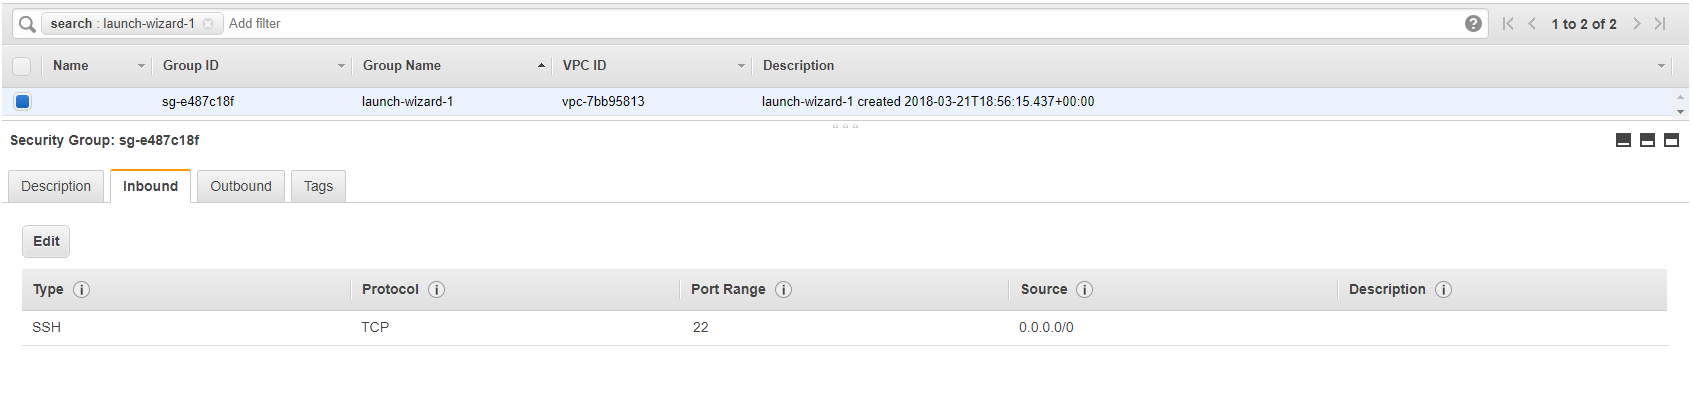
\includegraphics[width=160mm, scale=1]{Images/AWS_default_security_group_rules.PNG}
      \caption{AWS EC2 Default Security Rules} 
      \medskip
	  \small
		The default security group associated with an AWS EC2 instance when it is launched. The only security rule that is defined for this security group is SSH access over port 22/TCP from all IPv4 addresses.
\label{fig:DefaultEC2SecurityRules}
\end{figure}

%\includewidefigure{DefaultEC2SecurityRules}{AWS EC2 Default Security Rules}{The default security group associated with an AWS EC2 instance when it is launched. The only security rule that is defined for this security group is SSH access over port 22/TCP from all IPv4 addresses.}{Images/AWS_default_security_group_rules.PNG}
% TODO update with a snip


\subsection{The Cowrie Honeypot: A First Look}
By installing and configuring a plain Cowrie honeypot on the deployed AWS EC2 instance, it would be possible to understand the basic setup and configuration of the Cowrie honeypot before attempting to encapsulate it in a container environment. This was the next step undertaken in understanding the details of how the proposed system would be implemented.

\subsubsection{Installing Cowrie}    \label{InstallingCowrie}
As discussed in \textit{Section \ref{AboutCowrie}}, the Cowrie honeypot is an emulated of a Debian installation written in Python. A comprehensive installation guide for the Cowrie honeypot is provided on the Cowrie Github page. \cite{CowrieInstallationInstructions} By following this guide, it was relatively straight-forward to set up a Cowrie honeypot running as a Python \textit{virtualenv}\footnote{Python \textit{virtualenv} is a tool for creating isolated Python environments. It is used in Cowrie to create a virtual honeypot environment. \cite{VirtualEnvReference}}. The crucial requirement was to ensure that Cowrie is run by a non-root user, since it should be difficult for an attacker to achieve privilege escalation if they manage to interface directly with the host environment. Cowrie provides a safety net in this regard: If one was to attempt to launch the honeypot as a root user, it will fail to launch and output the log message \textit{'ERROR: You must not run cowrie as root!'}

The most significant configuration step in this process was to enable Cowrie to receive attack traffic destined for the EC2 host instance. By default, Cowrie listens for incoming traffic on ports 2222/TCP and 2223/TCP of its host, and thus for it to receive traffic from privileged ports 22/TCP (SSH) and 23/TCP (telnet)  some level of traffic forwarding was required. There are two approaches to achieving this recommended in the Cowrie installation guide: \cite{CowrieInstallationInstructions}

\begin{enumerate}
\item \textbf{Port Forwarding} 

Port forwarding involves using \textit{iptables} rules to forward incoming traffic on ports 22/TCP (SSH) and 23/TCP (telnet) to ports 2222/TCP and 2223/TCP.

\item \textbf{Direct Listening using Authbind}

As privileged ports, listening directly to incoming traffic on 22/TCP and 23/TCP requires root-user privileges. Cowrie will not run with such privileges, and so the \textit{authbind} Linux utility can be used to allow it to listen directly to traffic on these ports.

\end{enumerate}

In this initial installation of the Cowrie honeypot, listening as non-root using the \textit{authbind} utility was the approach taken.

The last step in this process is to update the configuration of the SSH daemon on the host instance so that it is still externally accessible by administrators. This is required since all incoming traffic on the default SSH port 22/TCP is now being forwarded to Cowrie, and involved a simple edit to the \textit{/etc/ssh/sshd\_config} file, changing the \textit{Port} value from 22/TCP to a different available port number. 



\subsubsection{Configuring Cowrie}
There are three primary components of Cowrie that can be used to customise the honeypot environment.
    \begin{itemize}
    \item \textit{\textbf{userdb.txt}}

    This file is used by Cowrie to determine what username-password combinations the honeypot should accept from an attacker. The default values for a clean Cowrie installation can be seen in figure \ref{fig:userdb_default}.
    
    \begin{figure}[ht]
      \centering
      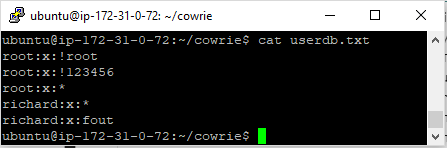
\includegraphics[width=160mm, scale=0.6]{Images/userdb_default_screenshot.PNG}
      \caption{Cowrie Honeypot Default Passwords} 
      \medskip
	  \small
		This image shows the default username-password combinations that are provided in Cowrie's \textit{userdb.txt} file. The first entry \textit{root:x:!root} specifies that username \textit{root} should be accepted, but not when the password specified is also \textit{root}. The third entry \textit{root:x:*} specifies that username \textit{root} should be accepted, with any other passwords for which there is no rule specified.
\label{fig:userdb_default}
\end{figure}
    
   % \includewidefigure{userdb_default}{Cowrie Honeypot Default Passwords}{This image shows the default username-password combinations that are provided in Cowrie's \textit{userdb.txt} file. The first entry \textit{root:x:!root} specifies that username \textit{root} should be accepted, but not when the password specified is also \textit{root}. The third entry \textit{root:x:*} specifies that username \textit{root} should be accepted, with any other passwords for which there is no rule specified.}{Images/userdb_default_screenshot.PNG}
    \item \textit{\textbf{cowrie.cfg}}

    This file is the main configuration file that is used by Cowrie to determine how to set up the honeypot environment. It comes with a multitude of settings, including parameters for integration with external tools\footnote{Currently, the external tool support for Cowrie listed on the Github repository README is listed as follows: Cuckoo Sandbox, ELK stack, Graylog, Kippo-Graph, Splunk, SQL (MySQL, SQLite3, RethinkDB). \cite{CowrieGithub}} and other parameters to control how the honeypot environment appears to an attacker. 
\item \textbf{honeyfs/}

It is possible to configure the file system contents of the honeypot environment through the addition of files and directories to the \textit{honeyfs/} directory. 
    \end{itemize}
    
    For this initial investigation into the operation of Cowrie, the configuration of all of  these components were left almost completely unaltered with default values.


\subsubsection{Exposing the Honeypot to Attacks}
\label{ExposingCowrieToAttack}
In order to understand the logging data produced by Cowrie, the honeypot was set up and exposed to the public internet. The installed Cowrie honeypot was configured with a name corresponding to a particular model of TPLink IP camera\footnote{The TPLink-TL-SC3171 model was chosen, since upon conducting a brief web search this model was immediately identified as having a Remote Code Execution (RCE) vulnerability: A highly desirable target. \cite{TPLinkIPCameraRCE}}, devices which are commonly targeted by IoT botnets. The default EC2 security group was left unaltered, meaning that the honeypot was exposed to the entire IPv4 address space on port 22/TCP (SSH). 

The environment was exposed for 1 hour, and in that time logged brute-force authentication attacks from 4 different IP addresses. These attacks were identified to be  bot attacks\footnote{Based on the timestamps logged by Cowrie, subsequent login attempts were spaced broadly 1 second apart: A speed which would be difficult for a human attacker to achieve consistently, leading to the classification of these attacks as bot attacks.} whose source IP addresses were identified to be from multiple different countries including Egypt, Russia, China and Vietnam\footnote{The source location was determined by using \textit{Maxmind GeoIP Database} which approximates the geolocation of IP addresses. \cite{MaxmindGeoipDatabase}}. 

One of the attack sessions was of particular interest, since upon comparison of the attempted login credentials it was observed that several of the passwords were the same as those identified by Antonakakis \textit{et al.} in the source code of the Mirai botnet\footnote{A number of the default passwords observed by Antonakakis \textit{et al.} in their research can be seen in \textit{Section \ref{IoTBotnetsSoA}}. Of these, passwords \textit{admin}, \textit{7ujMko0admin}, \textit{1234}, \textit{admin1234}, \textit{default}, \textit{password} were passwords in common with the bot attack observed here. The highly unusual password \textit{7ujMko0admin} would appear to indicate that this attack was conducted by a device that had been compromised by Mirai or one of its variants.}. \cite{UnderstandingTheMiraiBotnet} This was an interesting find, and illustrates the sheer scale of the infection of devices by this botnet and its variants.

The Cowrie log, which captured the attack session data in JSON format, gave an insight into the level of detail of information that Cowrie can capture. The information captured in these sessions included:

\begin{itemize}
\item The source IP and port of the connection;
\item The remote SSH protocol version and encryption algorithm used;
\item The username-password combinations that were attempted, and whether the attempt succeeded or failed;
\item How long the connection was maintained for, and the reason why the connection was terminated\footnote{For example, this could be something like too many incorrect login attempts, in which case the message ''too many bad auths'' would be logged by Cowrie.};
\item Timestamps corresponding to each event, and a unique session ID per connection.
\end{itemize}

As information that would later be processed by the ELK stack tools in the incident monitoring system, seeing the level of detail of JSON logging provided by Cowrie was useful towards understanding what visual data could potentially be generated from honeypot logs.

%
%	Building Docker Containers (Experimentation)
%

\subsection{Building Docker Containers}
The Docker ecosystem is straight-forward in principle, but is composed of a number of distinct components that together enable the stateless hosting of applications in containers. Understanding the components of this ecosystem and how they interoperate would be essential to effectively using this technology to implement the honeynet.

The basic Docker-Cowrie source code provided by the Cowrie Project \cite{DockerCowrie} was used to understand the construction of container environments and how to interoperate them before progressing to the implementation of the containerised honeynet.

\subsubsection{Docker Images}
A Docker container environment is completely specified by its image definition. This image definition can be defined using a \textit{Dockerfile}. The Dockerfile defines what the environment inside a container looks like, and consists of a set of text commands that are used to build the image\footnote{The full set of commands that can be specified in a Dockerfile can be found in the Docker documentation. \cite{AllCommandsForDockerfiles}}. Any external files referred to within the Dockerfile form part of the \textit{build context} of the image.

The lifecycle of a container is often referred to as the \textit{build-and-run} cycle, illustrated in figure \ref{fig:DockerBuildAndRun}\footnote{This illustration is adapted from a diagram in a presentation given by the authors of the paper \textit{Using Docker Containers to Improve Reproducibility in Software and Web Engineering Research.} \cite{ReproducableResearchEnvironmentsContainers} \cite{DockerBuildAndRunDiagram}.}.

\begin{enumerate}
\item \textbf{Building a Docker Image}

By issuing the \textit{docker build} CLI command with reference to a Dockerfile, a container image is generated by the Docker engine using the Dockerfile and the build context. The instructions in the Dockerfile are executed one-by-one and committed incrementally to the new image before finally generating an ID for the image. The new image usually uses a \textit{base image} as a foundation, which is a top-level image upon which other images can be built.

\item \textbf{Running a Docker Container}

If the \textit{docker create [arguments] [image-ID]} CLI command is issued with reference to an image ID, a writeable container layer is created based on that image and is prepared for running using any arguments provided. The resulting container layer is tagged with a container ID. However, the container is not automatically launched after being created: Issuing a \textit{docker start [container-ID]} CLI command will launch the container.

If instead the \textit{docker run [arguments] [image-ID]} command is issued with reference to the image ID, the same writeable container layer is created and the container is immediately launched. 

\item \textbf{Stopping or Removing a Container}

After being launched, a container can be stopped using the \textit{docker stop [container-ID]} command. The container can also be removed using the \textit{docker container rm [container-ID]} command, but only if either (i) it is not running, or (ii) it is running but the removal is forced by specifying additional arguments.

\end{enumerate}

    \begin{figure}[ht]
      \centering
      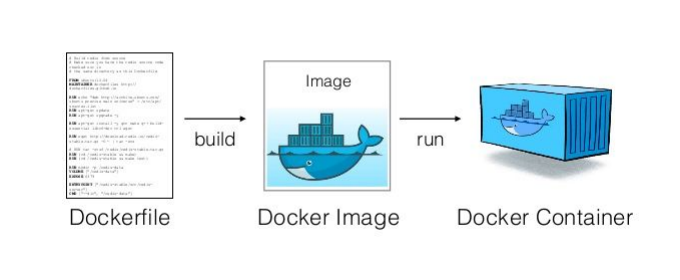
\includegraphics[width=160mm, scale=1]{Images/Docker_build_and_run_cycle.png}
      \caption{The Docker \textit{build-and-run} Cycle} 
      \medskip
	  \small
		An adapted illustration of the Docker \textit{build-and-run} cycle. The Dockerfile is used to build a Docker image, which in turn is used to run a Docker container.
\label{fig:DockerBuildAndRun}
\end{figure}

%\includewidefigure{DockerBuildAndRun}{The Docker \textit{build-and-run} Cycle}{An adapted illustration of the Docker \textit{build-and-run} cycle. The Dockerfile is used to build a Docker image, which in turn is used to run a Docker container.}{Images/Docker_build_and_run_cycle.png}


\subsubsection{Entrypoint Scripts}
Different elements of a container environment must be configured at particular points in the container lifecycle: Certain configuration options can be specified pre-runtime, whilst others must be specified at runtime. For example, one cannot update a container's internal routing table until that container is actually running, and hence this configuration cannot be directly specified as part of the static Docker image. This seems a nuisance since it means that not all environment configuration can be directly defined within the container image, but it is here that the use of the Docker \textit{ENTRYPOINT} command becomes useful.

The \textit{ENTRYPOINT} command can be used in a Dockerfile to specify a script which should be run when a container using that image is launched. This means that in the previous example, a script defining updates to the container's internal routing table can be specified as the \textit{ENTRYPOINT} command in the Dockerfile. After launching the container, this script will be executed and the routing table will be updated. This is a useful and flexible option in the configuration of a container environment.

%- Needed to be able to allow non-root container user to write to a docker volume directory.

\subsubsection{Docker Volumes} \label{DockerVolumesExperimentation}
Docker volumes were discussed in \textit{Section \ref{PersistingDockerContent}} as a means of persisting volatile content generated by a container. They can be mounted by using the \textit{VOLUME} command in the Dockerfile for a container image, and the corresponding host directory to which they are mapped is specified as an argument to the \textit{docker create} or \textit{docker run} CLI commands at a later stage. Once a container is stopped, any volumes that are mounted to it and their contents are persisted: It is only when the container is completely removed that the volume is also removed.

Figure \ref{fig:DockerVolumes} shows a conceptual view of how volumes can be used to persist content generated within a container, on the host system. 

    \begin{figure}[ht]
      \centering
      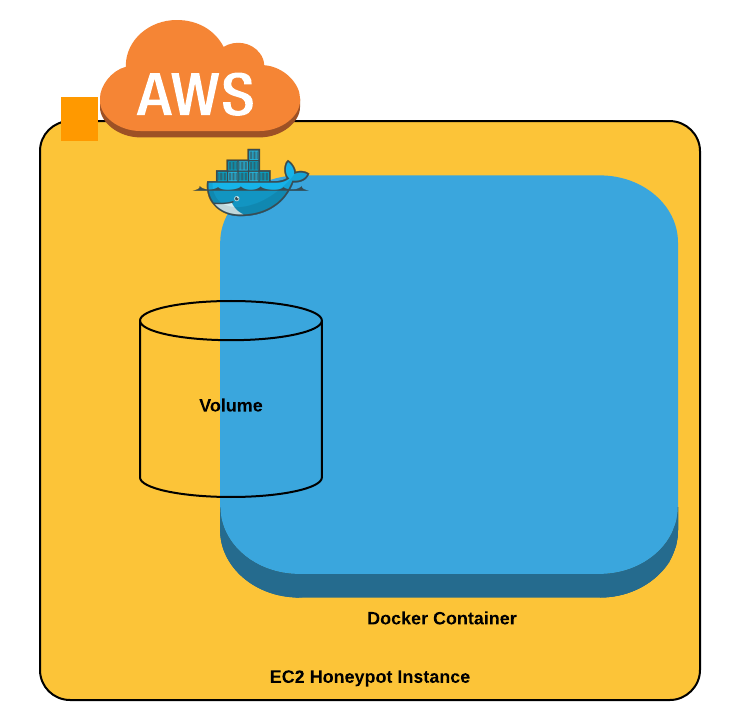
\includegraphics[width=125mm, scale=1]{Images/Another_illustration_of_how_a_Docker_volume_looks.png}
      \caption{A Conceptual Representation of Docker Volumes} 
      \medskip
	  \small
		A conceptual view of how Docker volumes operate. Files in this volume are accessible both from the host and the container in a specific directory on each system. Changes can be made dynamically to the contents of either directory and are immediately available in the corresponding mapped directory. 
\label{fig:DockerVolumes}
\end{figure}

%\includewidefigure{DockerVolumes}{A Conceptual Representation of Docker Volumes}{A conceptual view of how Docker volumes operate. Files in this volume are accessible both from the host and the container in a specific directory on each system. Changes can be made dynamically to the contents of either directory and are immediately available in the corresponding mapped directory. }{Images/Another_illustration_of_how_a_Docker_volume_looks.png}


\subsubsection{Docker Networking}
    Containers, like a physical machine, have their own networking stack. Each container has its own ports, and can have virtual interfaces connecting them to virtual Docker networks. This is the key piece of functionality that makes Docker so well-suited to the implementation of the honeynet in the proposed system.
    
    There are two different ways of exposing ports through the \textit{docker create} and \textit{docker run} CLI commands, which have different effects. 
\begin{itemize}

\item Using the \textit{--expose} argument exposes the specified container port to the host machine and to other containers. It is not however published to the host's network interfaces.

\item On the other hand, using the \textit{--publish} argument publishes the specified container port to the host's network interfaces meaning that it is accessible through these ports on the public internet.
\end{itemize}

An \textit{EXPOSE} argument can also be specified in the Dockerfile of an image, meaning that when a container is built from that image the specified ports are exposed for \textit{inter-container communication} only.  This is the default option specified in the Docker-Cowrie Dockerfile built by the Cowrie Project developers. \cite{DockerCowrie}

All containers, unless a network is otherwise specified, are automatically connected to a default Docker bridge network\footnote{As explained in the Docker documentation, \cite{UseBridgeNetworksDocker} ''a bridge network is a Link Layer device which forwards traffic between network segments... In terms of Docker, a bridge network uses a software bridge which allows containers connected to the same bridge network to communicate.''} called \textit{bridge} once created. This network allows the containers to communicate directly with each other and with the host machine through a virtual network interface called \textit{docker0}. Additional networks can be manually defined as bridge or overlay\footnote{An overlay network is described in the Docker documentation as ''a distributed network among multiple Docker daemon hosts. This network sits on top of (overlays) the host-specific networks, allowing containers connected to it ... to communicate securely. \cite{UseOverlayNetworksDocker} } networks. 

\subsection{Conclusions} \label{ConclusionsToExperimentationSection}
%Anything in relation to the use of these tools together.
Having explored the operation of AWS EC2, the Cowrie honeypot and the Docker container ecosystem, a solid understanding and some basic configuration had been achieved regarding the next steps in the implementation of the research environment described in \textit{Chapter 4}.  In particular, by the time all of the aforementioned Docker functionalities had been explored a rudimentary deployment script named \textit{do\_honeypot.sh} had been developed for the rapid removal and deployment of containers. This script could, based on simple parameters, perform functions including:

\begin{itemize}
\item Building the basic Docker-Cowrie image;
\item Creating a container based on the pre-built image, given a unique container name;
\item Launching and stopping a container given its name;
\item Entering a running container, presenting an internal container CLI to the user;
\item Providing usage instructions on how to use the script to manage containers on the system.
\end{itemize}

This, coupled with the knowledge gained about the operation of Cowrie and AWS EC2, formed a solid starting point from which to begin implementing the research environment.



%% 
%% SECTION 2: Host Server Setup
%%


\section{Host Server Deployment} \label{HostServerSetup}

There were two AWS EC2 server instances deployed for the implementation of the system: A honeypot server instance and a management server instance, as designed in \textit{Chapter 4}. The same deployment process described in \textit{Section \ref{DeployingAnAWSEC2Instance}} was followed. Both instances were hosted in the Amazon US East (Ohio) availability zone\footnote{As explained in the AWS EC2 documentation, ''Amazon EC2 is hosted in multiple locations world-wide. These locations are composed of regions and Availability Zones. Each region is a separate geographic area. Each region has multiple, isolated locations known as Availability Zones.'' \cite{WhatAreAWSAvailabilityZones}} running Ubuntu 16.04 LTS operating systems. Each instance was allocated different hardware resources depending on their requirements. In both cases, the hardware requirements were such that those provided by the AWS 12-month free tier were not sufficient, meaning that more expensive cost-incurring instances were needed.

\subsection{The EC2 Honeypot Server Instance}
	
	In order to host a number of Docker containers as part of the proposed containerised honeynet, a relatively powerful server instance was required. Based on the initial experimentation with running Docker containers on the free-tier instance, an EC2 instance with 16GB RAM and 4 virtual CPUs was provisioned in order to allow multiple Docker containers to be hosted\footnote{The free-tier specifications of 2GB RAM were determined to be insufficient for hosting multiple Docker containers, since it was found that multiple Docker containers launched simultaneously would cease to run due to memory shortages.}. 
	
    To be able to attract the attention of IoT bots scanning the public internet for vulnerable devices, the SSH (22/TCP) and telnet (23/TCP) default ports needed to be visible on this server instance. In total, just these two ports were exposed to the entire public internet by configuring security rules\footnote{It was deemed unnecessary to allow access on other ports, since for the purpose of collecting data for experiments the activities of interest were limited to attacks over SSH and telnet as are typical of IoT botnets.}\textsuperscript{,}\footnote{During the initial development of the system, access to these two ports was restricted through the AWS EC2 security rules to a select IP address for testing purposes.}. 
    
    One other port was opened on the server instance but with greater access restrictions. As described in \textit{Section \ref{InstallingCowrie}}, the purpose of this port is to ensure that administrative access to this server instance would be maintained. The port was chosen at random as 45678/TCP, and was exposed only to the IP address of the management instance to obscure the fact that this port was open as much as possible.
    
All security rules configured for the honeypot server instance can be seen in figure \ref{fig:HoneypotInstanceSecurityRules}.

    \begin{figure}[ht]
      \centering
      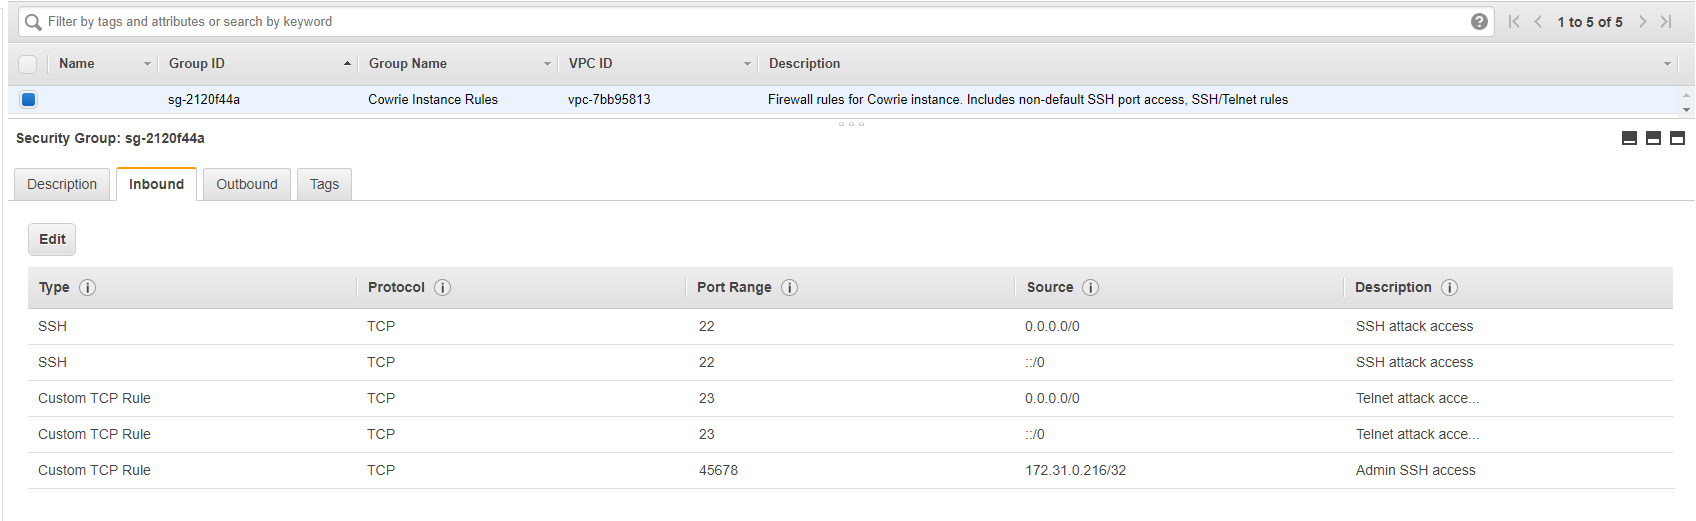
\includegraphics[width=160mm, scale=1]{Images/AWS_honeypot_instance_security_group_rules.PNG}
      \caption{AWS EC2 Honeypot Server Instance Security Rules} 
      \medskip
	  \small
		The 'Cowrie Instance Rules' security group, showing the rules defined for access to the AWS EC2 honeypot server instance. For each of SSH (22/TCP) and telnet (23/TCP), these ports were exposed to the entire IPv4 and IPv6 address spaces, whilst port 45678/TCP was only exposed to the IP address of the management server instance.
\label{fig:HoneypotInstanceSecurityRules}
\end{figure}

%\includewidefigure{HoneypotInstanceSecurityRules}{AWS EC2 Honeypot Server Instance Security Rules}{The 'Cowrie Instance Rules' security group, showing the rules defined for access to the AWS EC2 honeypot server instance. For each of SSH (22/TCP) and telnet (23/TCP), these ports were exposed to the entire IPv4 and IPv6 address spaces, whilst port 45678/TCP was only exposed to the IP address of the management server instance.}{Images/AWS_honeypot_instance_security_group_rules.PNG}
	
    
\subsection{The EC2 Management Server Instance} \label{DeployingTheManagementInstance}
    
	Since the management server instance was required to host the ELK log processing stack, there were certain minimum hardware resources required to be able to run these tools. Due to cost considerations, a minimal set of resources were allocated to meet the requirements: A server with 4GB of RAM and 2 virtual CPUs\footnote{The default RAM allocated to Elasticsearch, which is more resource-hungry than Logstash and Kibana, is 1GB. \cite{ElasticsearchHeapSizing} Upon the first installation of Elasticsearch on a server with 2GB RAM, it was found that this memory allocation was insufficient since Elasticsearch would continuously run out of heap memory. In a comprehensive tutorial by DigitalOcean which explains the steps required to configure these tools on an Ubuntu installation, 4GB of RAM was deemed sufficient. \cite{DigitalOceanELKTutorial} This led to the eventual decision to allocate a server with 4GB of RAM.} . The installation and configuration of the tools to be hosted on this EC2 instance are described later in \textit{Section \ref{LoggingAndVisualisationSection}}.

On this server instance, there were three ports which were exposed using security rules:
	\begin{itemize}
    	\item Port 22/TCP for SSH administrator access;
        \item Port 5045/TCP, which was a port randomly chosen to allow the honeypot server instance to transfer logs to the management server instance;
        \item Port 80/TCP, to allow HTTP access from a web browser to view the visualisations that would later be available from this server.
	\end{itemize}
    
 All security rules configured for the management server instance can be seen in figure \ref{fig:ManagementInstanceSecurityRules}.

 \begin{figure}[ht]
      \centering
      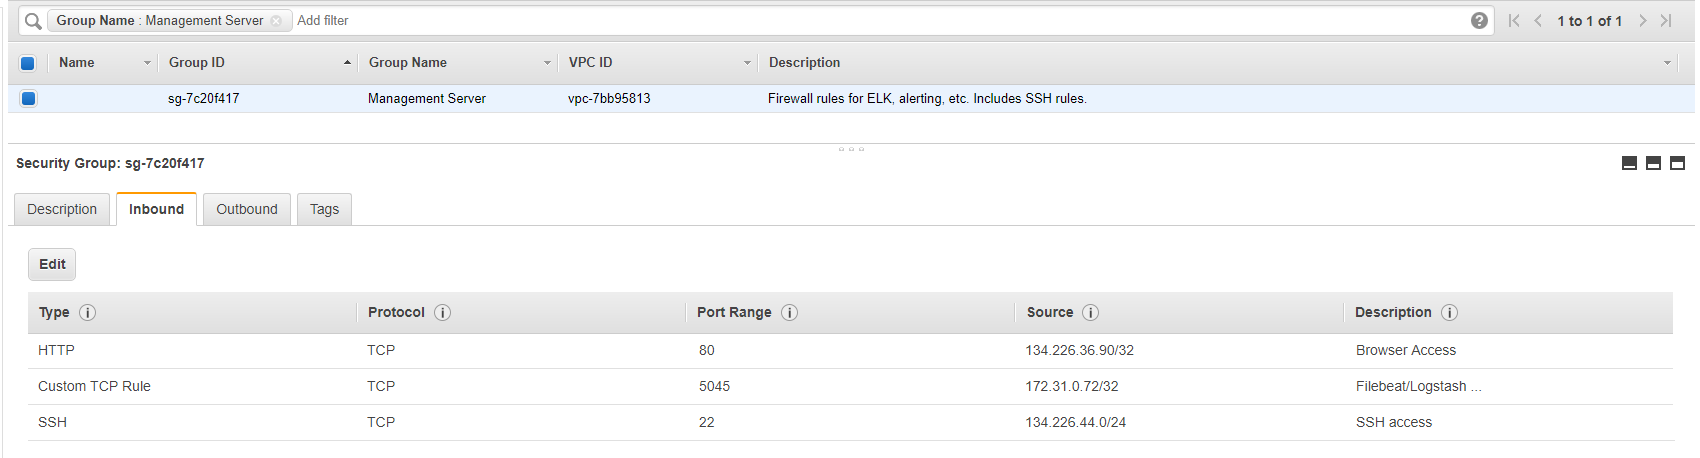
\includegraphics[width=160mm, scale=1]{Images/AWS_management_instance_security_group_rules.PNG}
      \caption{AWS EC2 Management Server Instance Security Rules} 
      \medskip
      \small
		The 'Management Server' security group, showing the rules defined for access to the AWS EC2 management server instance. Port 80/TCP here is seen to be exposed to a single IP address, from which access to the visualisations generated could be accessed via a web session. Port 5045/TCP is exposed to the IP address of the honeypot server instance to allow the Filebeat log-shipping application to transfer encrypted log files to the management server instance. Port 22/TCP is also exposed to a single IP address to allow administrative access to the instance.
\label{fig:ManagementInstanceSecurityRules}
\end{figure}

%\includewidefigure{ManagementInstanceSecurityRules}{AWS EC2 Management Server Instance Security Rules}{The 'Management Server' security group, showing the rules defined for access to the AWS EC2 management server instance. Port 80/TCP here is seen to be exposed to a single IP address, from which access to the visualisations generated could be accessed via a web session. Port 5045/TCP is exposed to the IP address of the honeypot server instance to allow the Filebeat log-shipping application to transfer encrypted log files to the management server instance. Port 22/TCP is also exposed to a single IP address to allow administrative access to the instance.}{Images/AWS_management_instance_security_group_rules.PNG}




%% 
%% SECTION 3: The Docker Honeynet
%%


\section{Building the Docker Honeynet\label{BuildingTheDockerHoneynet}}
One of the initial considerations that was described in \textit{Section \ref{EaseOfDeploymentDesignDecision}} was that the Docker honeynet should be deployable automatically by recording all commands required to build the networked environment in bash scripts. Throughout the development of the Docker honeynet described in this section, the \textit{do\_honeypot.sh} deployment script described in \textit{Section \ref{ConclusionsToExperimentationSection}} was incrementally expanded to include multiple functions and verbose output messages for easy deployment, removal and maintenance of the honeynet.

%
% COWRIE CONTAINER    
%
\subsection{The Cowrie Container}
It was decided in the design phase that the Docker image for the Cowrie honeypot containers would be heavily based off the existing image developed by the maintainers of the Cowrie Project, which had already been explored in the experimentation phase. \cite{DockerCowrie} This image definition provides a sound basis for building an enhanced Cowrie container image which can facilitate the inter-networking of multiple containers in a honeynet configuration.


\subsubsection{Building an Enhanced Docker Image}
The Dockerfile developed by the maintainers of the Cowrie Project performs the following operations when being built into an image:

\begin{itemize}
\item The \textit{debian:jessie-slim} base OS image is downloaded and used as a foundation for the container image.
\item All dependencies required by Cowrie are installed, most of which are build dependencies.
\item The Cowrie application is configured in accordance with the mandatory installation steps specified on the Cowrie Github repository, \cite{CowrieInstallationInstructions} before removing all unnecessary build packages.
\item A non-root user \textit{cowrie} is created, and set as the default user for the container.
\end{itemize}

The Dockerfile also specifies a command to launch Cowrie at runtime under the \textit{cowrie} user, as well as specifying a working directory \textit{/cowrie/cowrie-git/}, mounting two Docker volumes and exposing ports 2222/TCP and 2223/TCP, the default host ports on which Cowrie listens for incoming traffic. 

The creation of a default non-root user and removal of unnecessary build packages make the container environment suitably restrictive in the event that an attacker was able to bypass the Cowrie application and interface directly with the underlying container. Additional customisations were added to this base image definition to facilitate functions required by the Cowrie honeynet.

\subsubsection{Additional Linux Utilities}
The Cowrie application is capable of emulating many common Linux utilities including \textit{cat}, \textit{wget}, \textit{echo} and many others. As an open-source project it is even possible to add new utility emulations if desired. Thus, there are very few packages that actually need to be installed on the Cowrie container, and those that are required are mostly build dependencies. \cite{DockerCowrie} The only additional dependency required was \textit{authbind}, to allow Cowrie to receive incoming attack traffic from its host container. 

In the customised Cowrie Dockerfile, an \textit{entrypoint script} was specified to be executed at container runtime. This script was used to configure \textit{authbind} as in \textit{Section \ref{InstallingCowrie}} so that Cowrie could listen to traffic on ports 22/TCP (SSH) and 23/TCP (telnet) of the container. The script is shown in Snippet 5.1. \mbox{}\\ 
\mbox{}\\
\mbox{}
\linebreak

\includecode{Cowrie entrypoint script}{The entrypoint script specified in the customised Cowrie Dockerfile. This shows the configuration of \textit{authbind} by creating 2 new empty files using \textit{touch}, the assignment of ownership of these files to the \textit{cowrie} user, and full read-write-execute permissions being given to \textit{cowrie} user for both of these files. This allows the \textit{cowrie} user to use \textit{authbind} to receive incoming traffic on these ports. Cowrie then needs to be notified that \textit{authbind} is being used, achieved by setting the \textit{AUTHBIND\_ENABLED} configuration parameter. Finally, the script launches the Cowrie honeypot under the \textit{cowrie} user.}{Code_snippets/cowrie_listen_authbind.sh}\label{cowrie_entrypoint_script}


\subsubsection{Sharing and Persisting Container Data}
As identified in \textit{Section \ref{PersistingDockerContent}} and explored in \textit{Section \ref{DockerVolumesExperimentation}}, volumes are useful for dynamically sharing information between a container and its host. The use of volumes in the Cowrie containers in this system serves two purposes:

\begin{enumerate}
\item Cowrie configuration files can be specified on the host, and accessed by a container through a shared volume;
\item Logs generated inside a container by Cowrie can be accessed by the host through a shared volume, making them both accessible and persistent outside the container.
\end{enumerate}

Thus, in the honeynet deployment script an extended function was defined for the creation of Cowrie containers, specifying a number of volumes to be mounted to them.

\begin{itemize}
\item The \textit{dl/} directory in the Cowrie container was mounted as a volume to allow container access from the host. This is the default location where checksums of attempted downloads by attackers are stored.
\item The \textit{log/} directory in the Cowrie container was mounted as a volume to allow container access from the host. This is the default location where log files generated by Cowrie are stored.
\item The \textit{data/} directory in the Cowrie container was also mounted as a volume to allow host access from the container. This is the default location for the \textit{userdb.txt} password configuration file used by Cowrie.
\end{itemize}

As well as using volumes to make configuration files available inside Cowrie containers, the \textit{docker cp} command was used to copy the \textit{cowrie.cfg} file from the host into the container without using a volume\footnote{This was necessary because of an intricacy in the mounting of nested volumes from the host to a container: If the directory containing this file was mounted as a volume to the container, an issue would arise where the volumes corresponding to the nested \textit{/data}, \textit{/log} and \textit{/dl} directories would be overwritten.}. 


\subsubsection{Port Publication}
Because all containers need to be able to communicate with each other over ports 22/TCP and 23/TCP to enable the desired attack propagation between honeypots in the honeynet, the \textit{EXPOSE} command was used in the Cowrie Dockerfile. This meant that when launched, ports 22/TCP and 23/TCP on any Cowrie container would be visible to any other containers on the default Docker \textit{bridge} network.

In the case of the honeywall Cowrie container, the situation was slightly different: In order to be able to receive attacks, it needed to be able to access incoming traffic from the network interface of the host. To achieve this, when creating the honeywall container the \textit{--publish} argument was used to map ports 22/TCP and 23/TCP on the host network interface to the corresponding ports on the container. The use of the \textit{--publish} argument also meant that the container would automatically be assigned a virtual network interface on the \textit{bridge} Docker network, such that it would be able to receive the incoming network traffic on these ports from the host instance. Figure \ref{fig:HoneywallPortPublication} illustrates how this looks conceptually.

 \begin{figure}[ht]
      \centering
      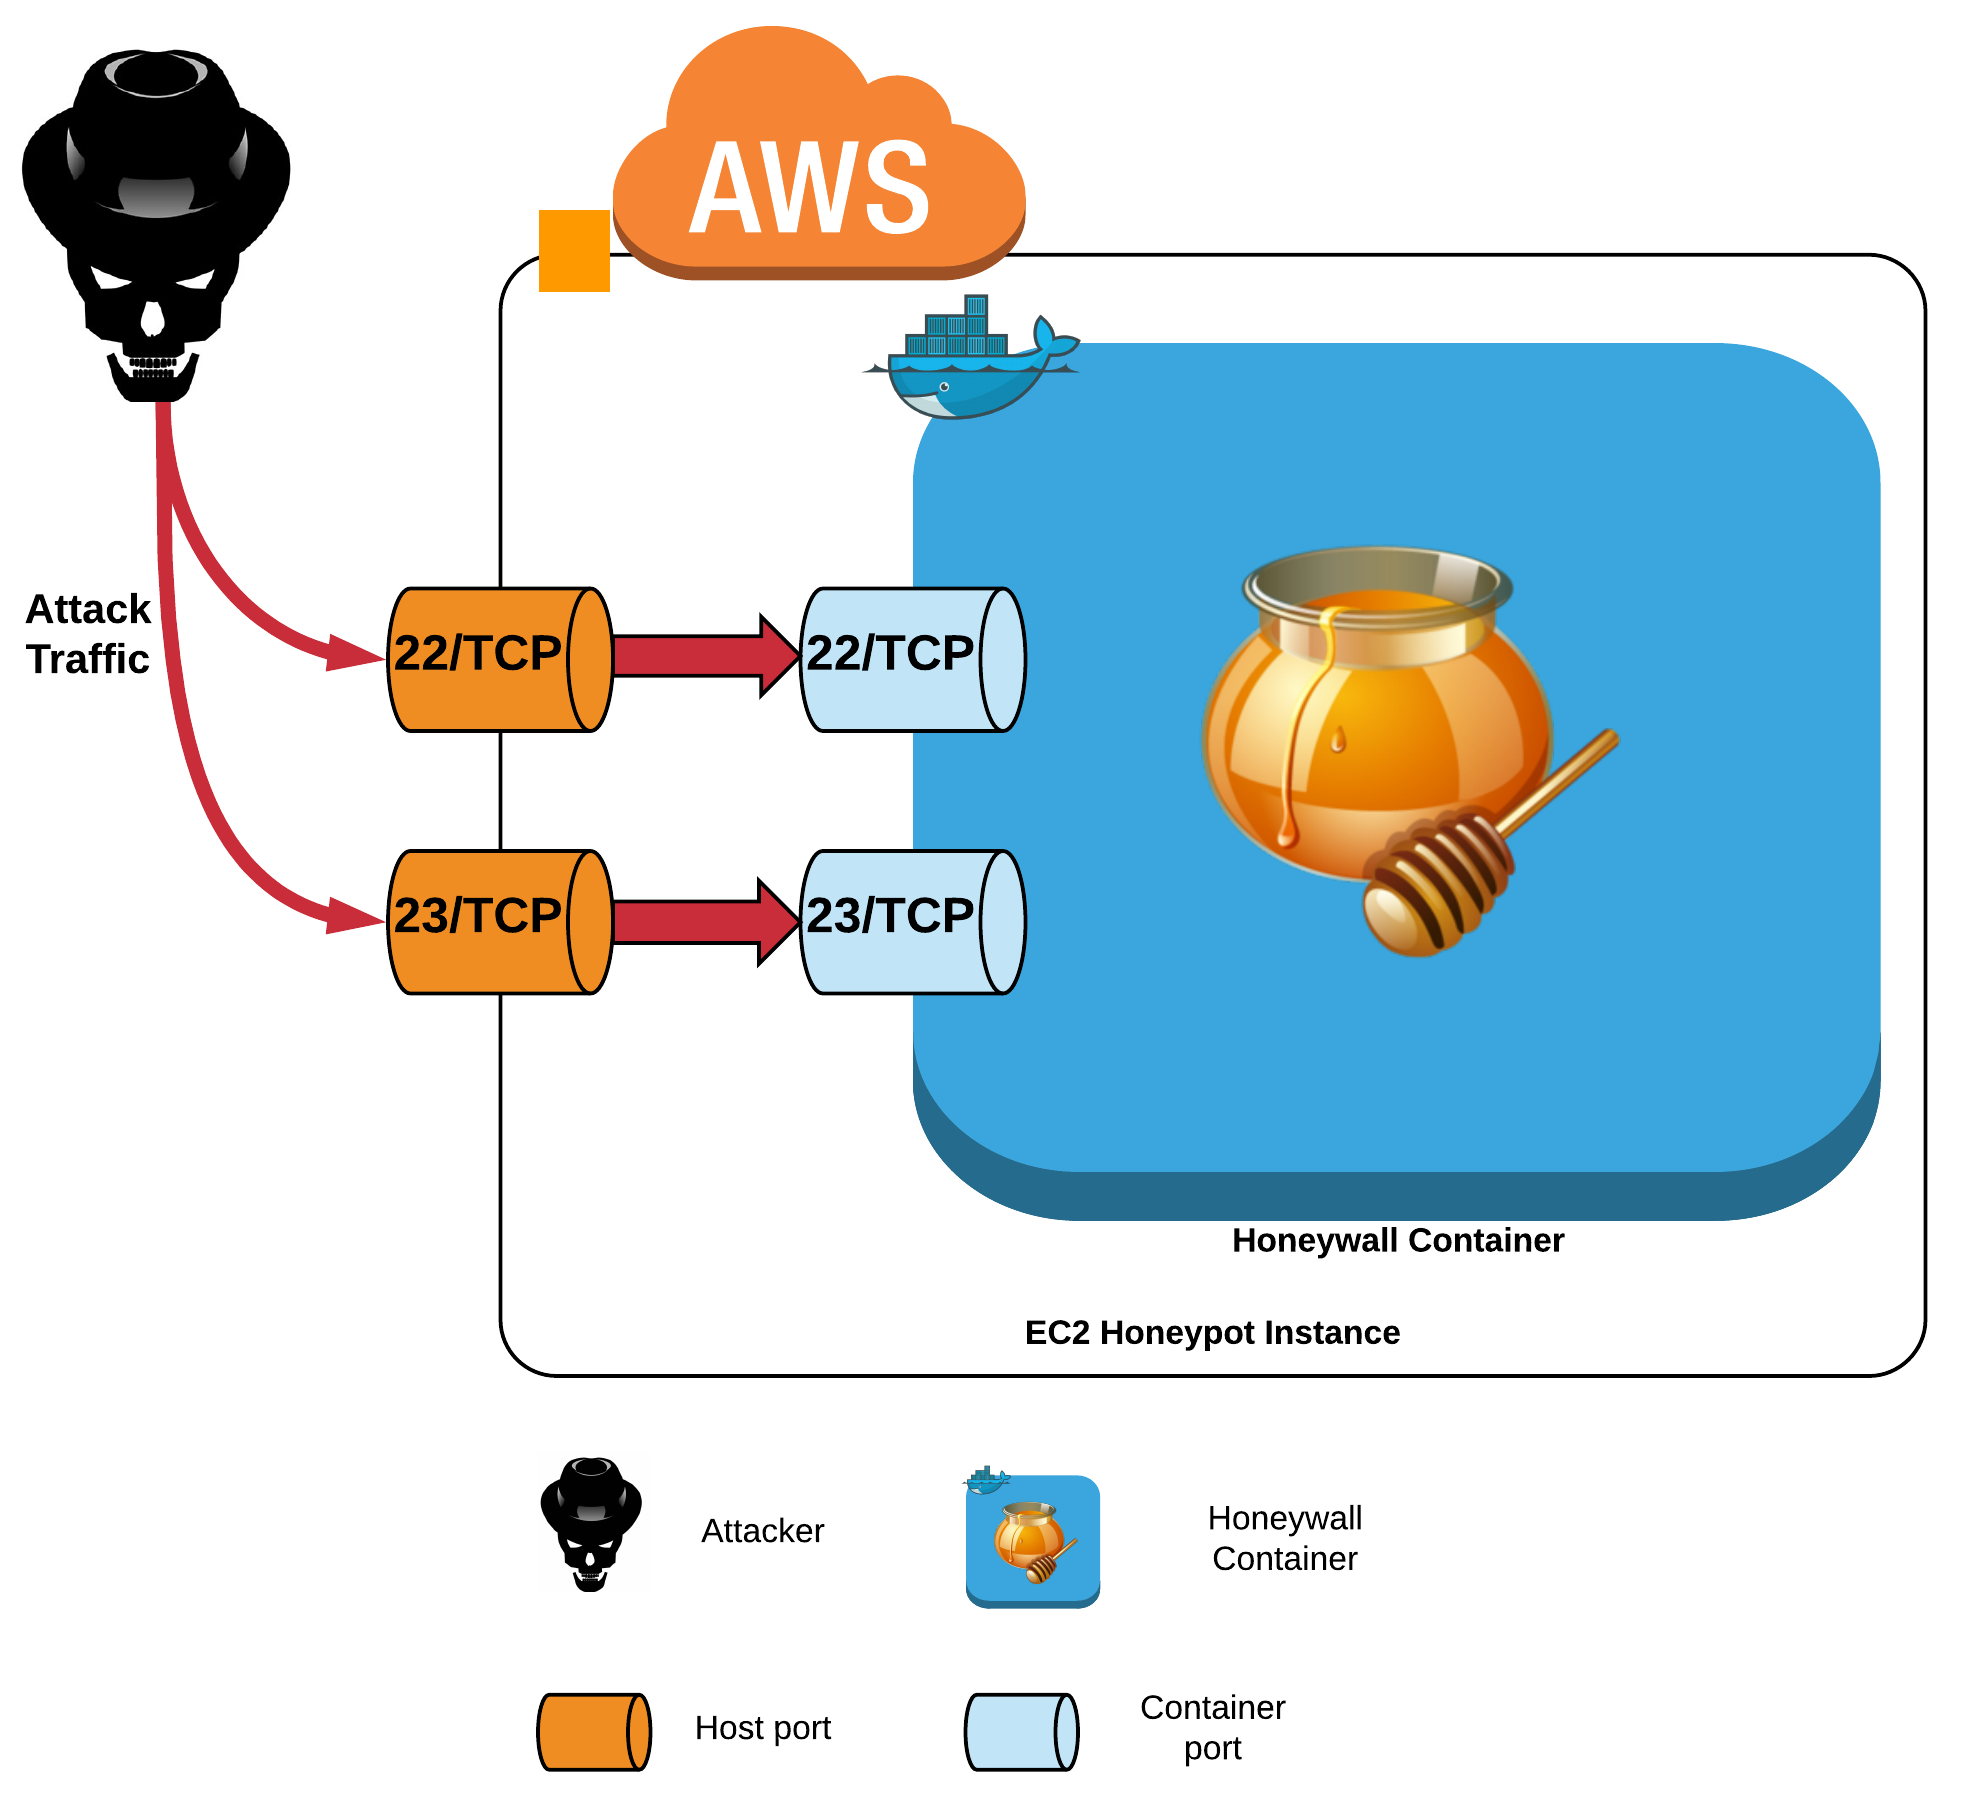
\includegraphics[width=125mm, scale=1]{Images/Port_mapping_for_the_honeywall_container.png}
      \caption{Port Publication on the Honeywall Container} 
      \medskip
      \small
		An illustration of the publication of ports 22/TCP, 23/TCP on the honeywall container to ports 22/TCP, 23/TCP on the host. Any traffic received by the host on these ports is mapped directly to the corresponding ports on the container, essentially making these container ports directly available from the Internet.
\label{fig:HoneywallPortPublication}
\end{figure}

%\includewidefigure{HoneywallPortPublication}{Port Publication on the Honeywall Container}{An illustration of the publication of ports 22/TCP, 23/TCP on the honeywall container to ports 22/TCP, 23/TCP on the host. Any traffic received by the host on these ports is mapped directly to the corresponding ports on the container, essentially making these container ports directly available from the Internet.}{Images/Port_mapping_for_the_honeywall_container.png}

A separate function was added to the \textit{do\_honeypot.sh} script to create and launch this container as distinct from an ordinary Cowrie container which would not be publishing these ports. 





%
% DOCKER HONEYNET
%
\subsection{The Docker Honeynet}
The Docker honeynet is one of the novel components of the system design, and would consist of new Docker network with a number of Cowrie containers connected to it. The honeywall Cowrie container would act as a gateway between the EC2 honeypot instance and this Docker network, meaning that it would need to have virtual interfaces on both the \textit{bridge} Docker bridge network and the new Docker network hosting the other Cowrie containers.

\subsubsection{Defining a Docker Bridge Network}
    The new Docker network that would host the Cowrie honeypot containers was defined as a bridge network with address 10.0.0.0/8\footnote{A /8 subnet can have up to 16,777,214 nodes with different IPv4 addresses. Though this scale is certainly not required here, the fact that these subnets are supported in Docker allows for many containers to belong to a single network.}. This network address was chosen because it is an address reserved for use in private networks, i.e. those not directly connected to the public internet. \cite{rfc1918}  The network was given the name \textit{dmz} corresponding to the notion of a DMZ explained in \textit{Section \ref{MotivationsForIntrusionDetection}}.
    
    In the \textit{do\_honeypot.sh} deployment script, a new function was added to allow a user to automatically define this network without needing to provide configuration details. This function can be seen in \textit{Snippet 5.2}.
    \mbox{}\\
    \includecode{Script to Create the Docker DMZ Network}{This script shows the commands used to create the virtual Docker bridge network, \textit{dmz}. The script uses the \textit{docker network ls} command to check whether the network already exists, and if not creates it. The \textit{-d bridge} argument specifies that the Docker bridge network driver should be used to create the network, and the \textit{attachable} argument indicates that containers can be added to the network manually on-the-fly.}{Code_snippets/create_dmz_net.sh}\label{create-dmz-net-code}

\subsubsection{Connecting Containers to the Honeynet}
% Specify IP addresses for everyone on the network
% What is the visibility of each container on the network? What ports are open (22, 23) and who can see that?
    
    As discussed in \textit{Section \ref{DockerSecurityConsiderations}}, ensuring that the honeypot containers did not have any unnecessary networking capabilities needed to be considered in the implementation. By specifying that Cowrie containers should be connected to the \textit{dmz} network as part of the \textit{do\_honeypot.sh} deployment script, they would not be added to any other networks by the Docker engine, ensuring this. 
    
    Connecting these containers to the \textit{dmz} network involved adding a single extra argument to the \textit{docker create} CLI commands for the Cowrie and honeywall containers in the \textit{do\_honeypot.sh} script: \textit{--network ''dmz''}. When executed, the \textit{docker create} command would now randomly assign an IP address on the \textit{dmz} network to the Cowrie containers, and a specific IP address to the honeywall container\footnote{The address 10.0.0.254/8 was specified for the honeywall container, since this address is commonly configured as the address for routing devices in real-world networks and so was determined to add to the attractiveness of this container from an attackers perspective.}. 
   

\subsubsection{Network Configuration of the Honeywall Container}
The function of the honeywall Cowrie container differs from that of other Cowrie containers in that it should act as a gateway between the Cowrie honeynet and the EC2 host. This requires that the honeywall Cowrie container have two virtual network interfaces: One on the default \textit{bridge} network in order to communicate with the host instance, and the other on the \textit{dmz} honeynet.

Configuring the honeywall container as the gateway for the \textit{dmz} network was not as easy to achieve as it first seemed. The issue encountered was as follows:
    \begin{itemize}
    \item The IP address of the network gateway must be specified at the time of creation of the network. It is not possible to specify a network component as the gateway, i.e. the honeywall container cannot be specified as the gateway, but in theory its IP address could be.
\item Clearly, a container cannot have an IP address for a network that has not already been created: Thus, a container cannot first be given an IP address and then that IP address specified as the gateway during the creation of the network.
    \end{itemize}
    
    In essence, it is not possible through Docker to the honeywall container as the gateway for the \textit{dmz} network, since the network must already be defined with a gateway before the container can be a part of it in the first place. As an issue for which no reference documentation existed, overcoming this issue took substantial troubleshooting and trial-and-error. Eventually, it was resolved by manual manipulation of the \textit{iptables} rules and routing table configuration once the container was running.
    
    To ensure that this configuration would always be present when this container is launched in future,  a new Dockerfile was created for the honeywall container. The Dockerfile contained the same configuration options as that of the other Cowrie containers, but used a different entrypoint script at runtime that would configure the \textit{iptables} rules and routing tables.


\subsection{Design Pivot: A New High-Interaction Honeypot}\label{DesignPivot1}
     
    It was discovered during the configuration of the honeywall container that the Cowrie honeypot does not have outbound networking capabilities such that it can make outbound SSH or telnet connections. This was something that was not fully understood about the Cowrie honeypot initially\footnote{It was understood before beginning the implementation of the system that the Cowrie honeypot \textit{did} have this functionality, since it is known that issuing a \textit{wget} download request inside the Cowrie honeypot downloads the requested resource and computes its SHA-checksum whilst appearing to the attacker to have failed. Such functionality would require the honeypot to make an outbound network connection, and the same approach was assumed to have been taken to the implementation of the SSH and telnet services in Cowrie.}, unearthed through implementation issues and verified by the maintainer of the Cowrie honeypot, Michel Oosterhof. In response to an email query on the subject, he outlined the following:
    
\begin{center}
''\textit{Cowrie by design doesn't do any outbound connections from within the honeypot... So if you want communicatoin between the instances, that'll be a fairly significant programming exercise. You'll need to learn some Python/Twisted and basically implement an SSH/Telnet client inside Cowrie that can connect to the next instance. Or you'll have to create some way to bypass this and make it appear that this is what happens to the attackers.}''
\end{center}    

When this realisation was made, the original approach to implementing the honeynet required immediate re-evaluation. The ability to make outbound network connections from the honeywall container is essential so that an attacker can access the honeynet. However, the honeywall container should also be a maximally restricted environment to minimise the risk of attack propagation outside of the system. These considerations motivated a re-assessment of the system design.

\subsubsection{Re-Evaluation of Initial Design \label{DesignReEvaluation}}
Given the time within which the research was being conducted, it would not be possible to extend the Cowrie source code to give the honeypots the ability to make outbound network connections over SSH and telnet. Instead, a decision was made to implement a new high-interaction Docker honeypot\footnote{It was decided to implement an entirely new high-interaction honeypot since there are very few high-interaction honeypots that exist, and none that were found to be actively maintained. In their survey of honeypot software, Nawrocki \textit{et al.} found that the majority of honeypot solutions are low-interaction, and that when it comes to high-interaction solutions ''only few exist''. \cite{Nawrocki2016}} to facilitate the propagation of attacks beyond the honeywall: A component referred to hereafter as the \textit{router container}. 

As a high-interaction honeypot, the router container faced an array of new challenges.

\begin{itemize}
\item Since attackers would no longer be interacting with an emulated environment inside the Docker container, real libraries and toolkits would have to be made available to encourage them to interact with the system.
\item The Cowrie application gives a simple configuration option for specifying username-password combinations that should be allowed or disallowed for authentication by the honeypot. This is not so easy to replicate in a real system, where a user account can only be configured to accept either (i) a single correct password\footnote{This also presents an additional issue, since if only a single correct password is permitted per user the probability of an attacker actually attempting this password is low.} or (ii) no password to authenticate a login. 
\item Attackers will always seek to gain root access to a system in order to have unrestricted control over it. Cowrie emulates this root access effectively, but this cannot be falsified in a real system and would require giving real root privileges to the attacker\footnote{This would be required since if attackers are not permitted to login as root, it is less probable that any attackers will ever reach the Cowrie honeynet.}. This is highly risky, since there is no limitation on what actions they can then perform inside the system.
\item An approach to logging network traffic and command execution would need to be identified in order to capture attack data, since these capabilities of the Cowrie honeypot would also no longer be available to this container.
\end{itemize} 

The approaches taken to deal with each of these new difficulties are detailed in the subsequent sections.

\subsubsection{Defining a New Container Image}
Since the requirements of the router container would be significantly different to that of the highly-restricted Cowrie container, a new Docker image definition was required. 

It was decided that in order to have access to a wide variety of powerful Linux utilities\footnote{This variety would be required to facilitate an attacker in accessing whatever utilities they required in order to progress with their attack: It would be undesirable for the attacker to disconnect from this container without progressing to the Cowrie honeynet, since experimental data would then never be captured by the honeynet.}, the \textit{ubuntu:latest} Docker base OS image would be used as a foundation for the router container image. The container would also need to expose ports 22/TCP and 23/TCP as with the Cowrie containers, and so these were specified in the Dockerfile using the \textit{EXPOSE} command.

The most generic Linux utilities that were specified as part of the Docker-Cowrie image were also included in this new image: In particular, the \textit{apt-utils} and \textit{build-essential} packages, which are required as basic utilities in almost all Debian-based Linux environments.

Once the basic Dockerfile was defined, the \textit{do\_honeypot.sh} script was updated to use the new router container image instead of the old honeywall container image. The \textit{docker create} arguments for adding the container to the \textit{dmz} network and publishing ports 22/TCP and 23/TCP to the host interface were left unchanged, since the router container would still require this configuration.

\subsubsection{Configuring SSH and Telnet}
Since there was now no emulation of SSH and telnet connectivity, it was necessary to install and configure utilities for these on the router container. The installation of the required packages was specified as part of the router container Dockerfile, and their runtime configuration properties specified in an entrypoint script.

\paragraph{SSH}\mbox{}\\
The installation of the \textit{openssh-server} utility was specified in the Dockerfile. Then, the entrypoint script was used to update the configuration of the SSH daemon \textit{sshd} to facilitate SSH logins to the container. Some noteworthy configurations specific to enabling easy access by attackers to the container include the following:

\begin{itemize}
    \item The \textit{PermitRootLogin} field was updated to allow SSH logins as user \textit{root};
    \item The \textit{PasswordAuthentication} field was updated to allow authentication by password and not just by using an encryption key;
    \item The \textit{PermitEmptyPasswords} field was updated to allow authentication with an empty password, if this was valid for a particular user.
\end{itemize}

Lastly, the entrypoint script was updated to restart so that the updated configuration would take effect.

\paragraph{Telnet}\mbox{}\\
The installation of the \textit{telnet}, \textit{openbsd-inetd } and \textit{telnetd} package utilities were also added to the Dockerfile. A number of configuration steps were also added in the entrypoint script to be applied at container runtime: In particular, the allocation of a number of \textit{ttys}\footnote{In Linux systems, a tty is a representation of a text input/output device to the system, such as a terminal session.} to allow multiple simultaneous telnet sessions to take place. 

A telnet configuration file called \textit{telnet} was also added to the container, which included a number of essential configuration options as well as some logging parameters. This required use of the Dockerfile \textit{COPY} command to copy the file into the container's \textit{/etc/xinetd.d} directory. As with the configuration of SSH, the telnet daemon is restarted to allow the changes to take effect.

\subsubsection{Device Banner Configuration}
As part of the \textit{enumeration} phase of an attack, an attacker will often use a scanning tool such as \textit{Nmap} or \textit{Masscan} to fingerprint the target system. These scanning tools usually send a message probe over particular protocols with the intention of receiving an acknowledgement (ACK) from the target, allowing the attacker to deduce some properties of the system. In the case of IoT devices, being able to fingerprint the device type and model is very useful to an attacker in identifying a vulnerable target, and so the router container needed to be capable of presenting such information.

There are two primary messages that are presented to those initiating a user authentication connection with a Linux-based system: The \textit{issue.net} and \textit{mot.d} files.
\begin{itemize}
\item \textbf{issue.net / issue}

        This file is used to set the banner that is sent in a protocol negotiation, e.g. for a client requesting to connect to the system via telnet, this would be the information that is used to greet the client prior to the login step. For SSH, this file is called \textit{issue} whereas for telnet the file is called \textit{issue.net}.

\item \textbf{motd / legal}

        This file is used to display a message to a client after they have successfully logged into the system. Often, administrators will use this to present a notice about permitted uses of the system after a user has successfully logged in. For SSH, this file is called \textit{legal} whereas for telnet the file is called \textit{motd}.
		\end{itemize}
        
In the Dockerfile for the router container, commands were added to copy customised \textit{issue.net}, \textit{issue}, \textit{legal} and \textit{motd} files defined on the host into the container. Some additional updates were then made to the entrypoint script so that these banners would be presented in connection negotiations. Figure {fig:router-telnet-banner} shows how these banners appear to an individual attempting to gain access to the system via telnet.

 \begin{figure}[ht]
      \centering
      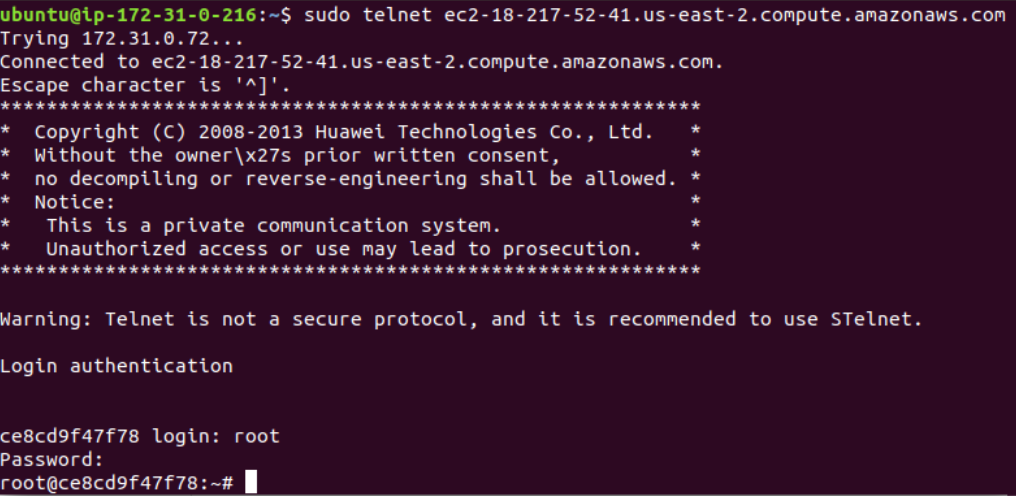
\includegraphics[width=160mm, scale=1]{Images/logging_into_router_container_with_telnet.PNG}
      \caption{The Router Container Honeypot Telnet Banner} 
      \medskip
      \small
		This screenshot shows a login attempt via Telnet to the EC2 honeypot server instance. It can be seen that a banner advertising a Huawei device is presented as part of the login prompt. It can be observed that the ''attacker'' proceeds to successfully log in as user \textit{root}.
\label{fig:router-telnet-banner}
\end{figure}

%\includewidefigure{router-telnet-banner}{The Router Container Honeypot Telnet Banner}{This screenshot shows a login attempt via Telnet to the EC2 honeypot server instance. It can be seen that a banner advertising a Huawei device is presented as part of the login prompt. It can be observed that the ''attacker'' proceeds to successfully log in as user \textit{root}.}{Images/logging_into_router_container_with_telnet.PNG}

\subsubsection{Privileges and Authentication}
As identified in \textit{Section \ref{DesignReEvaluation}}, for an attacker to interact with the system they would need to believe that they have gained root-level access to the router container. This is not something that can be falsified without the use of an emulated environment like Cowrie, and so the decision was made to allow root access by default for all user accounts on this container. 

A related issue is the fact that arbitrary user-name password combinations could not be accepted in the same way on a real Linux environment as they could be with the emulated Cowrie environment. 
\begin{itemize}
\item In  order for an attacker to log in to the router container under a particular user, an account needs to exist for that user.
\item  As well as this, it is only possible to specify one valid password per user account.
\end{itemize} 
The reality of this was that the number of username-password combinations that could be accepted for this honeypot would be greatly restricted. 

The solution to these issues was to define a number of user accounts with usernames commonly observed in brute-force authentication attacks, and give each of these users root privileges by default. Since the exact username-password combinations used in the system would be determined through experiments, a single account for user \textit{admin} was created as part of the Dockerfile. 

In order to give root privileges to user accounts, they needed to be declared as \textit{sudo} users\footnote{A sudo user is one which has root privileges on the system, with unrestricted read, write and execute capabilities.}. This involved the installation of the \textit{sudo} package as part of the Dockerfile, and the use of the \textit{COPY} command in the Dockerfile to copy a pre-configured sudoers file into the container from the host. This sudoers file was configured such that it granted root-level privileges to the \textit{admin} user for all utilities in the container.


This configuration should now allow an attacker authenticated as user \textit{admin} to successfully carry out unrestricted activities inside the container.


\subsubsection{Logging Attack Events}
As with the Cowrie honeypot containers, it was essential that the router container could monitor the activities of an attacker on the system. This container is a high-interaction honeypot: A fully-fledged container with a real networking stack, toolkits and file system. As described in \textit{Section \ref{HoneypotInteractivityLevels}}, these honeypots offer the highest value in terms of capturing information about interactions with attackers since attacker activities are usually unrestricted. The most important elements of attack activities that needed to be captured in logging were the commands executed by attackers, and details of the attacker's connection session. 

 \paragraph{Network Event Logging}\mbox{}\\
  The most commonly used logging utility for network events is \textit{syslog}. Syslog is IETF standard Linux logging utility, which logs network and process events that occur on a system. It is heavily used by system administrators for system management and security auditing purposes. \cite{rfc5424} It was identified as a straight-forward logging solution for capturing information about attacker connections to the router container, since it is capable of capturing logging information for both SSH and telnet.
  
 In order to use syslog, the \textit{rsyslog} package was added to the Dockerfile as part of the image installation for the router container. A custom-defined configuration file called \textit{rsyslog.conf} was then added to the container image, and in the entrypoint script for the container the \textit{rsyslog} utility was launched\footnote{The launching of the \textit{rsyslog} utility was the last operation specified in the entrypoint script in order. This was to ensure that none of the environment configuration updates applied by the script were included in the log files, meaning that if an attacker was to inspect the syslogs on the container they would not see any records relating to the configuration of the environment, reducing the likelihood of them fingerprinting it as a honeypot.}. 
  
 In order to persist the logs generated by \textit{rsyslog} inside the router container, a volume was mounted to the router container in the \textit{/var/log} directory as part of the function to create the router container in the  \textit{do\_honeypot.sh} script. SSH and telnet events are logged to a number of different log files within this directory, including \textit{auth.log}, \textit{messages}, \textit{secure} and \textit{syslog}.
    

	  \paragraph{Keylogging}\mbox{}\\
      \textit{Logkeys} is an open-source Linux keylogger. \cite{LogkeysGithub} As one of the only identified Linux keyloggers freely available and relatively recently maintained, it was originally selected as a keylogging solution for monitoring the activities of attackers inside the router container.
      
      There were a number of significant difficulties encountered with the use of \textit{logkeys}: Seemingly, these were due to its incompatibility with Docker.
      % event interface of the Linux input subsystem
      \begin{itemize}
      \item There was no single reference which specified all of the dependencies required to be installed in order for \textit{logkeys} to operate. Since Docker containers take a lean approach to sharing libraries and packages with their host\footnote{In general, Docker base images such as the Ubuntu Docker image are shipped only with the bare minimum of packages included, and require a lot of additional packages to be installed in order to run and manage applications.}, many of these dependencies had to be installed from the \textit{apt} repositories. These dependencies were eventually identified through investigating \textit{dumpkeys}, an ancient Linux keylogger which shares a lot of the same library dependencies. \cite{dumpkeysKeyloggerManpage}
      \item The fact that \textit{logkeys} depends on being able to reference a keyboard device driver on the host machine presented a number of issues to the use of keylogging. Input device drivers are stored in Linux systems in a device file, which appears as an ordinary file under the \textit{/dev/input} directory. Although a \textit{--device} argument exists for the \textit{docker create} CLI command which can be used to reference a device driver on the host, the keyboard input device remained inaccessible by \textit{logkeys} inside the Docker container despite over a week of dedicated effort.
      \end{itemize}
 
 After exhausting all identified venues for implementing keylogging with \textit{logkeys}, a number of additional options were investigated.
 
 \begin{itemize}
 \item The idea of using the Linux \textit{.bash\_history} file for keylogging was explored. This file is created by the Bash utility, and captures all executed command-line inputs. This initially seemed a reasonable approach to keylogging: However, the fact that commands are not logged with timestamps would render the data largely unusable for identifying distinct attack sessions, making this an unsuitable approach.
 \item A manual keylogging approach was attempted, inspired by a recommendation on the online forum \textit{askubuntu.com}. \cite{ManualKeyloggingAskUbuntu} This keylogging approach involved using pure shell command manipulation, leveraging off SSH and telnet environment variables generated as part of \textit{syslog} network event logging. However, this approach was found to be unreliable and brittle, and so was also abandoned.
\end{itemize}
 
With the time constraints involved in the implementation of the system, the idea of keylogging was eventually put to one side as future work to improve the router container honeypot. 
     
\subsubsection{Package Utilities}
As identified in the design re-evaluation in \textit{Section \ref{DesignReEvaluation}}, a number of Linux utilities that an attacker would expect to find in a legitimate system needed to be made available  in the container, since the emulation of these utilities provided by Cowrie were no longer available. In particular, it was important to facilitate an attacker in probing the \textit{dmz} network in order to discover the Cowrie honeypot containers, and so providing common networking packages was a must.

The initial utilities that were added to the Dockerfile for the router container were \textit{net-tools}, \textit{nmap}, \textit{traceroute}, \textit{inetutils-ping}, \textit{iptables }and \textit{tcpdump}. These are all networking packages that would allow an attacker to perform actions such as viewing and manipulating the container's routing table, scanning nearby hosts and capturing packets on the network. 
   
\subsection{Finalising the Docker Honeynet}
Now that all required components of the Docker honeynet had been implemented, all that remained was to ensure that the network configuration was operating correctly. An attacker should be able access the router container from the public internet and from there, interact with any available Cowrie containers on the \textit{dmz} network. 

The targeted network configuration for the deployment is illustrated in figure \ref{fig:honeypot-instance-networking}.

\begin{figure}[ht]
      \centering
      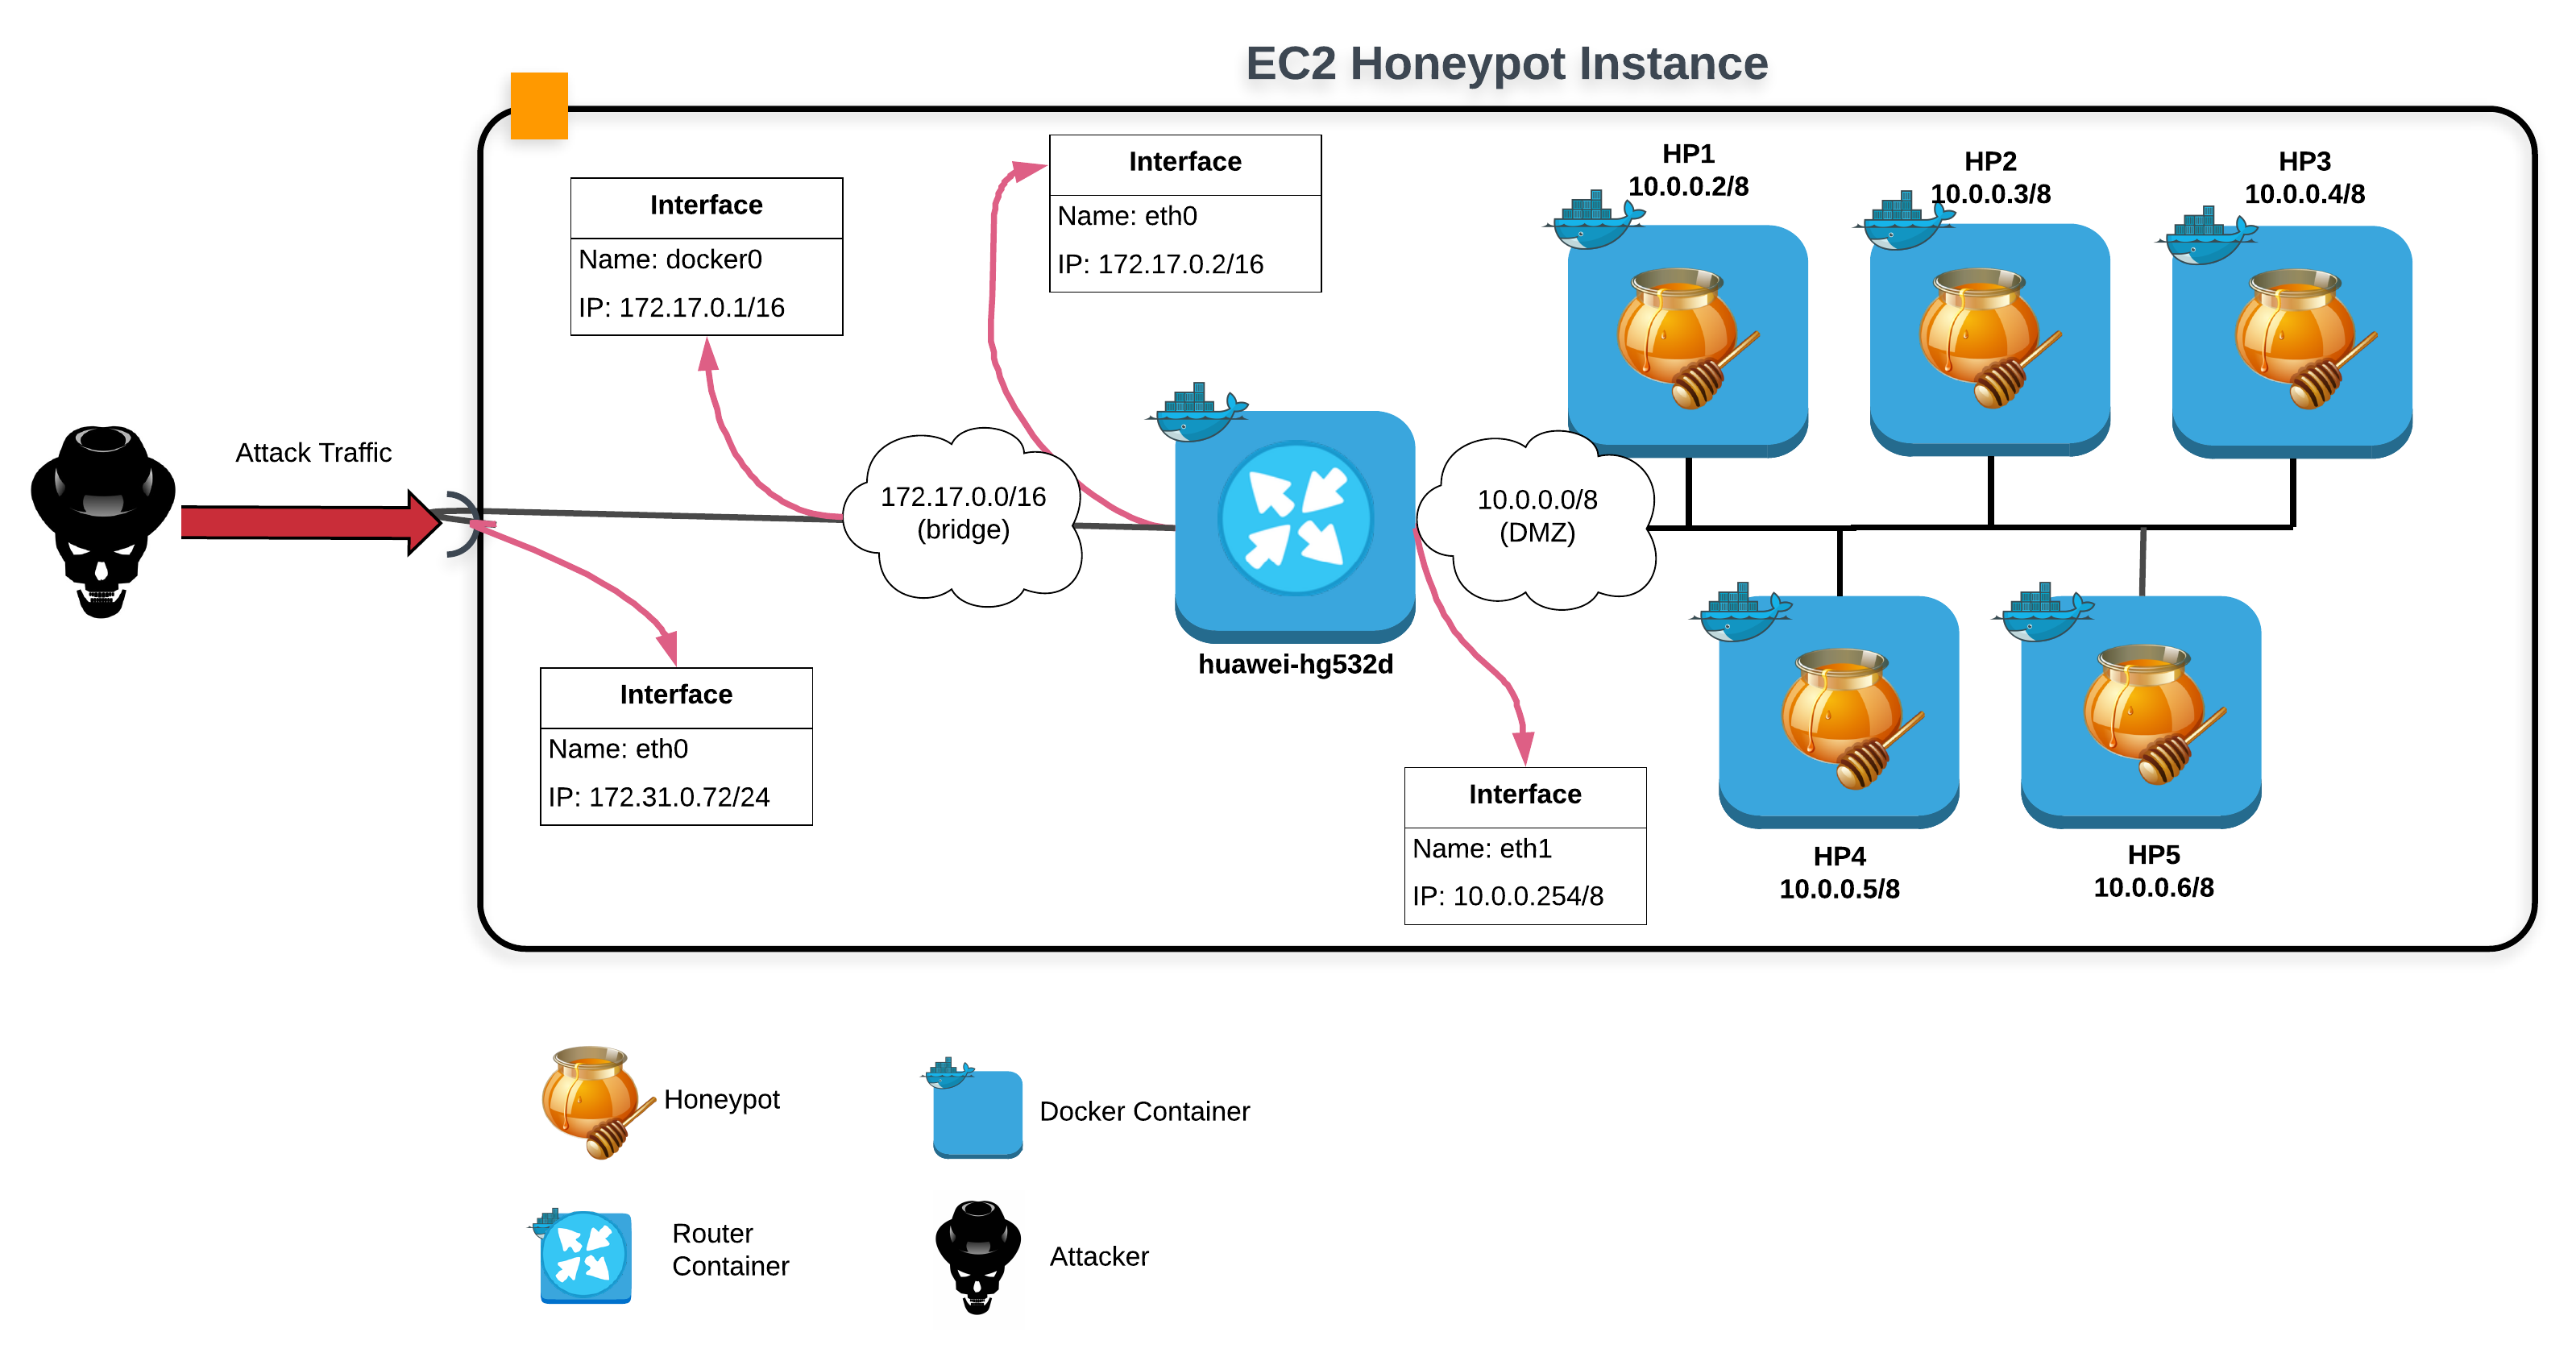
\includegraphics[width=160mm, scale=1]{Images/Honeypot_Instance_Networking.png}
      \caption{Docker Network Configuration of the EC2 Honeypot Instance} 
      \medskip
      \small
		This figure illustrates the desired network configuration for the honeynet deployment on the EC2 honeypot instance. It can be observed that there are two bridge networks: \textit{bridge} and \textit{dmz}. The host instance is forwarding its incoming traffic on ports 22/TCP and 23/TCP to the \textit{docker0} virtual interface on the \textit{bridge}. This interface connects the host to the router container's virtual interface \textit{eth0}. The router container also has a second virtual interface, \textit{eth1} which connects it to the \textit{dmz} network. It is through this interface that the Cowrie honeypots in the \textit{dmz} network can be accessed.
\label{fig:honeypot-instance-networking}
\end{figure}

%\includewidefigure{honeypot-instance-networking}{Docker Network Configuration of the EC2 Honeypot Instance}{This figure illustrates the desired network configuration for the honeynet deployment on the EC2 honeypot instance. It can be observed that there are two bridge networks: \textit{bridge} and \textit{dmz}. The host instance is forwarding its incoming traffic on ports 22/TCP and 23/TCP to the \textit{docker0} virtual interface on the \textit{bridge}. This interface connects the host to the router container's virtual interface \textit{eth0}. The router container also has a second virtual interface, \textit{eth1} which connects it to the \textit{dmz} network. It is through this interface that the Cowrie honeypots in the \textit{dmz} network can be accessed.}{Images/Honeypot_Instance_Networking.png}


\subsubsection{The Docker \textit{bridge} Network Configuration}
For the router container to be accessible from the public internet, its configuration on the \textit{bridge} Docker network needed to  be set up to facilitate this. The first step was to inspect the configuration of the \textit{bridge} network and the routing table on the EC2 instance itself. The desired configuration is illustrated in figure \ref{fig:router-container-config}.

\begin{figure}[ht]
      \centering
      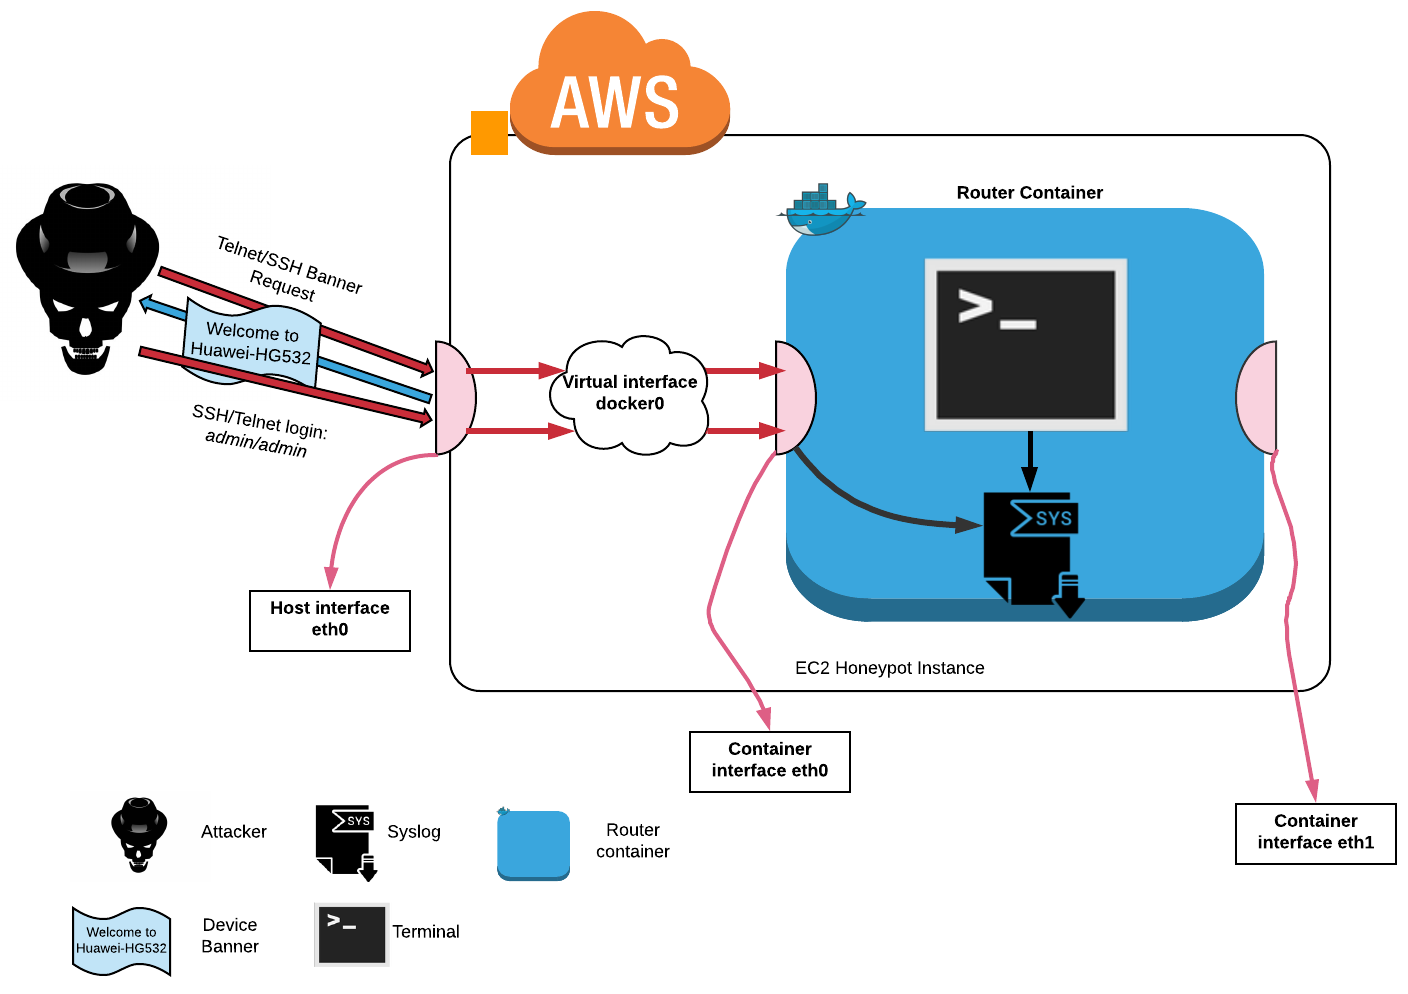
\includegraphics[width=160mm, scale=1]{Images/Router_container_config.png}
      \caption{Routing of Attack Traffic to the Router Container} 
      \medskip
      \small
		An illustration of the desired routing of attack traffic from the host network interface to the router container. The attacker is shown to attempt a brute-force authentication attack over either SSH or telnet, which is forwarded from the real host interface \textit{eth0} to the \textit{docker0} virtual interface on the \textit{bridge} network. From this interface, the traffic is forwarded to the \textit{eth0} router container interface. For the response to the attacker, the flow of traffic through the network is in reverse order through these interfaces. 
\label{fig:router-container-config}
\end{figure}

%\includewidefigure{router-container-config}{Routing of Attack Traffic to the Router Container}{An illustration of the desired routing of attack traffic from the host network interface to the router container. The attacker is shown to attempt a brute-force authentication attack over either SSH or telnet, which is forwarded from the real host interface \textit{eth0} to the \textit{docker0} virtual interface on the \textit{bridge} network. From this interface, the traffic is forwarded to the \textit{eth0} router container interface. For the response to the attacker, the flow of traffic through the network is in reverse order through these interfaces. }{Images/Router_container_config.png}

The internal routing table of the EC2 honeypot instance can be seen in table \ref{table:host-routing-table}, showing the networks associated with its physical network interface \textit{eth0} and Docker virtual network interface \textit{docker0}. By design, the host cannot interface directly with the \textit{dmz} bridge network: As discussed in \textit{Section \ref{DockerSecurityConsiderations}}, by preventing the host and containers from being connected to unnecessary networks the risk of these systems being compromised in an attack is minimised.

\begin{table}[!h]
	\begin{center}
		\begin{tabular}{|c|c|c|c|c|c|c|c|} 
			\hline
			\bf Destination  & \bf Gateway  & \bf Genmask  & \bf Flags & \bf Metric & \bf Ref & \bf Use & \bf Iface \\
			\hline
			0.0.0.0 & 172.31.0.1 & 0.0.0.0 & UG & 0 & 0 & 0 & eth0  \\
            172.17.0.0 & 0.0.0.0 & 255.255.0.0 & U & 0 & 0 & 0 & docker0  \\
            172.31.0.0 & 0.0.0.0 & 255.255.240.0& U & 0 & 0 & 0 & eth0  \\
			\hline
		\end{tabular}
	\end{center}
	\caption[Routing Table of the EC2 Honeypot Instance]{The routing table produced by the command \textit{route -n} executed on the honeypot instance, which hosts the Docker honeynet. Two interfaces can be observed: \textit{eth0} and \textit{docker0}. \textit{eth0} connects the host to the 172.31.0.0/24 network, which is an external network managed by AWS. The \textit{docker0} interface corresponds to a default bridge network called \textit{bridge} with address 172.0.0.0/16, which containers are connected to by default if not specified otherwise.}	
	\label{table:host-routing-table}
\end{table}

By executing the command \textit{docker network inspect bridge}, the properties of the Docker \textit{bridge} network can be inspected. The output of executing this command can be seen in figure \ref{fig:docker-network-inspect-bridge}. It can be seen that there is only 1 container on this network, corresponding to the router container \textit{router}. If the command \textit{docker container inspect router} is subsequently executed, the output obtained\footnote{The volume of output generated by this command is not feasible to include as a figure in this document, and so a description of the most important contents of the output was deemed sufficient.} demonstrates the following expected properties:

\begin{itemize}
\item The \textit{router} container is connected to the \textit{bridge} network with an IP address of 172.17.0.2/16;
\item The router container is also connected to the\textit{dmz} network with an IP address of 10.0.0.254/8;
\item Ports 22/TCP and 23/TCP of the \textit{router} container are published to ports 22/TCP and 23/TCP of the host interface.
\end{itemize}

\begin{figure}[ht]
      \centering
      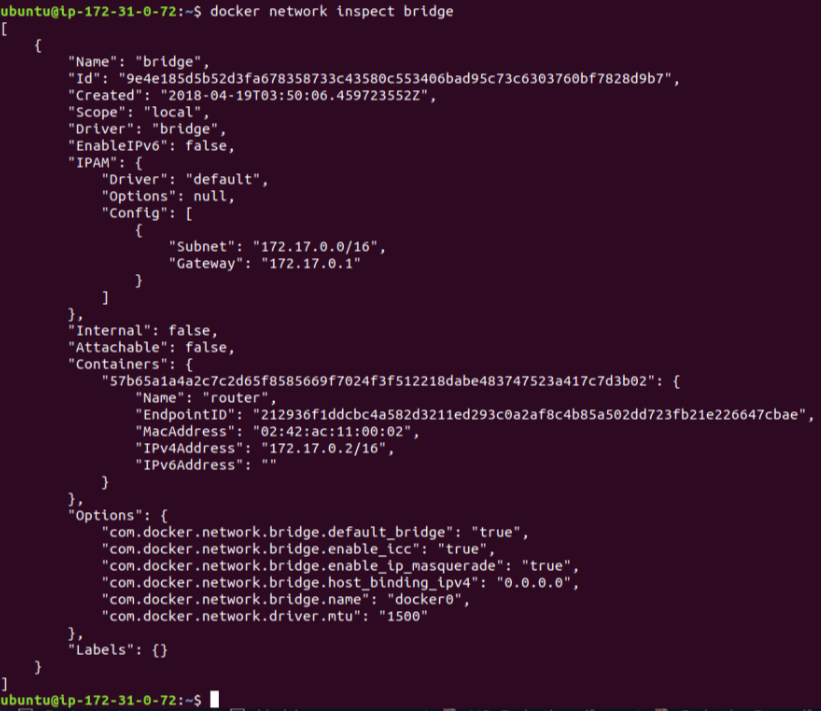
\includegraphics[width=160mm, scale=1]{Images/docker_network_inspect_bridge.PNG}
      \caption{Console Output of \textit{docker network inspect bridge}} 
      \medskip
      \small
		An image showing the console output obtained by executing the command \textit{docker network inspect bridge}. It can be observed that there is only 1 container on this network: The \textit{router} container. 
\label{fig:docker-network-inspect-bridge}
\end{figure}

The correct routing of attack traffic through the \textit{bridge} network could be tested from outside the EC2 honeypot server instance, by connecting over SSH or telnet to the instance and verifying that the router container login prompt is presented. Figure \ref{fig:ssh-to-router-successful} shows the console output when an SSH connection is made to the EC2 honeypot server instance, demonstrating the correct routing of this traffic to the router container.

\begin{figure}[ht]
      \centering
      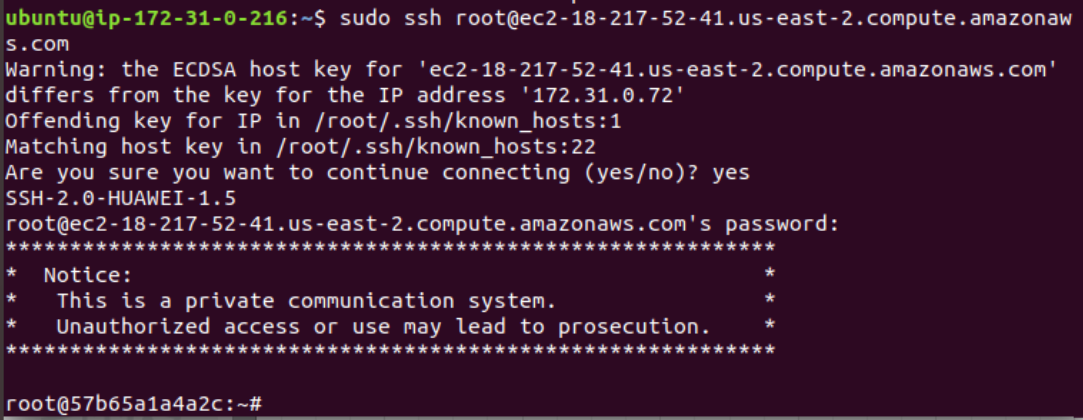
\includegraphics[width=160mm, scale=1]{Images/ssh_to_router_successful.PNG}
      \caption{Attempted SSH Login to the Router Container} 
      \medskip
      \small
		An image showing the console output obtained when a connection attempt is made over SSH to the EC2 honeypot instance. It can be observed that a Huawei banner is presented, and that the attacker is permitted to log in as \textit{root}. 
\label{fig:ssh-to-router-successful}
\end{figure}





\subsubsection{The Docker \textit{dmz} Network Configuration}
To verify that attack traffic could reach the Cowrie containers in the \textit{dmz} network,  the configuration of the router container and the \textit{dmz} network needed to be verified. An attacker, once inside the router container, should be able to connect through an interface on the router container to any Cowrie container on the \textit{dmz} network. The desired configuration is illustrated  in figure \ref{fig:cowrie-honeynet-container-config}.

\begin{figure}[ht]
      \centering
      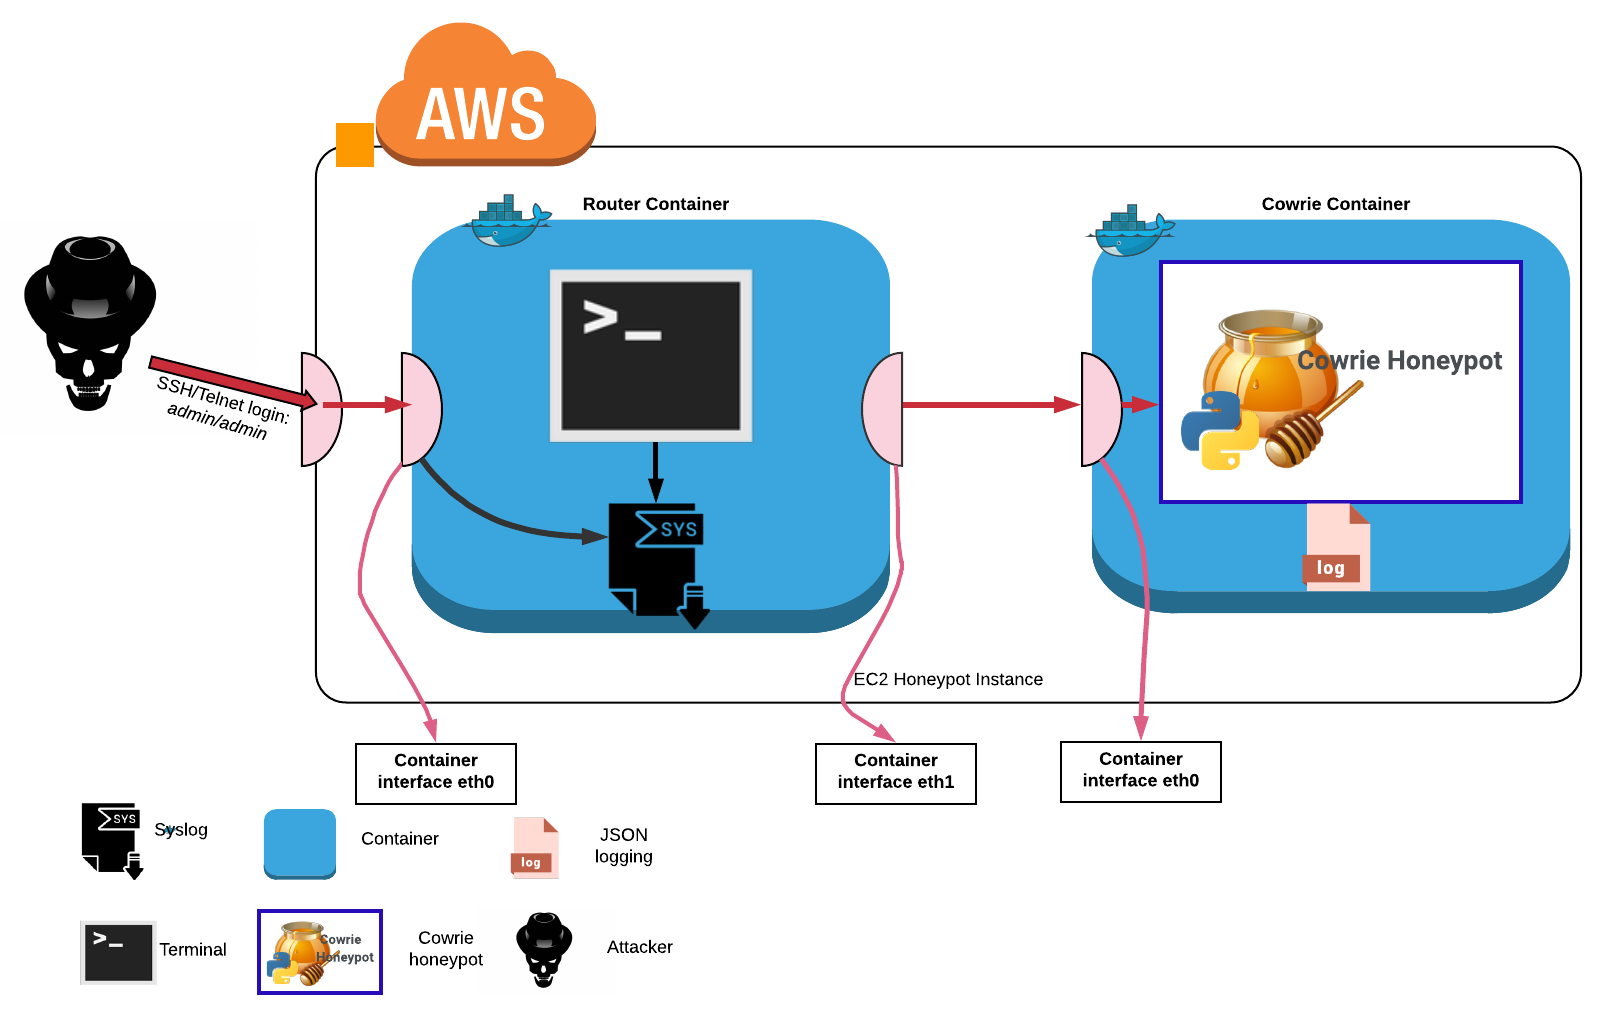
\includegraphics[width=160mm, scale=1]{Images/Cowrie_container_config.png}
      \caption{Routing of Attack Traffic to a Cowrie Container} 
      \medskip
      \small
		An illustration of the desired routing of attack traffic from the host network interface to a Cowrie container. Assuming that the attacker has already successfully compromised the router container through the process in figure \ref{fig:router-container-config},  they should be able to connect to the Cowrie container over SSH or telnet in the same way through the router container's \textit{eth1} interface on the \textit{dmz} network. 
\label{fig:cowrie-honeynet-container-config}
\end{figure}

%\includewidefigure{cowrie-honeynet-container-config}{Routing of Attack Traffic to a Cowrie Container}{An illustration of the desired routing of attack traffic from the host network interface to a Cowrie container. Assuming that the attacker has already successfully compromised the router container through the process in figure \ref{fig:router-container-config},  they should be able to connect to the Cowrie container over SSH or telnet in the same way through the router container's \textit{eth1} interface on the \textit{dmz} network. }{Images/Cowrie_container_config.png}[HD]

The internal routing table of the router container can be seen in table \ref{table:router-routing-table}, showing the networks associated with the container's two virtual interfaces \textit{eth0} and \textit{eth1}. These networks correspond to the \textit{bridge} network 172.17.0.0/16 and the \textit{dmz} network 10.0.0.0/8.

\begin{table}[!h]
	\begin{center}
		\begin{tabular}{|c|c|c|c|c|c|c|c|} 
			\hline
			\bf Destination  & \bf Gateway  & \bf Genmask  & \bf Flags & \bf Metric & \bf Ref & \bf Use & \bf Iface \\
			\hline
			0.0.0.0 & 172.17.0.1 & 0.0.0.0 & UG & 0 & 0 & 0 & eth0  \\
            10.0.0.0 & 10.0.0.254 & 255.0.0.0 & U & 0 & 0 & 0 & eth1  \\
            172.17.0.0 & 0.0.0.0 & 255.255.0.0 & U & 0 & 0 & 0 & eth0  \\
			\hline
		\end{tabular}
	\end{center}
	\caption[Routing Table of the Router Container]{The routing table produced by the command \textit{route -n} executed inside the router container. Two interfaces can be observed: \textit{eth0} and \textit{eth1}. \textit{eth0} connects the router container to the 172.17.0.0/16 \textit{bridge} network, whereas \textit{eth1} connects it to the 10.0.0.0/8 \textit{dmz} network.}	
	\label{table:router-routing-table}
\end{table}

From inside the router container, an attacker should be able to access a domain on the public internet in order to perform downloads to progress their attacks on the system. This is achieved through the configuration of Network Address Translation (NAT) rules in \textit{iptables}. The rules shown in snippet 5.3 were used to achieve this objective, enabling an attacker to perform downloads from external domains. This temporarily caused a diffiult-to-diagnose issue with the \textit{iptables} of the EC2 instance\footnote{The issue manifested as an inability to connect to containers on ports 22/TCP and 23/TCP, where Nmap would show these ports as being 'filtered'.}, which was eventually resolved by executing the command \textit{iptables -t nat --flush} to remove some conflicting NAT rules on the host.

\includecode{NAT iptables Rules}{The \textit{iptables} rules that were configured to enable NAT inside the router container.}{Code_snippets/NAT_iptables_rules.sh}\label{lst:nat-rules}

The routing table generated inside a Cowrie container can be seen in table \ref{table:cowrie-container-routing-table}. In this case, the container is connected to only one network: The \textit{dmz} network, which it accesses through its virtual interface \textit{eth0}.

\begin{table}[!h]
	\begin{center}
		\begin{tabular}{|c|c|c|c|c|c|c|c|} 
			\hline
			\bf Destination  & \bf Gateway  & \bf Genmask  & \bf Flags & \bf Metric & \bf Ref & \bf Use & \bf Iface \\
			\hline
			0.0.0.0 & 10.0.0.254 & 0.0.0.0 & UG & 0 & 0 & 0 & eth0  \\
            10.0.0.0 & 0.0.0.0 & 255.0.0.0 & U & 0 & 0 & 0 & eth0  \\
			\hline
		\end{tabular}
	\end{center}
	\caption[Routing Table of the Cowrie Container]{The routing table produced by the command \textit{route -n} executed inside a Cowrie container. One interface can be observed: \textit{eth0}. \textit{eth0} connects the container to the 10.0.0.0/8 \textit{dmz} network.}	
	\label{table:cowrie-container-routing-table}
\end{table}	
	
By executing the command \textit{docker network inspect dmz}, the properties of the Docker \textit{dmz} network can be inspected. The output of executing this command can be seen in figure \ref{fig:docker-network-inspect-dmz}. It can be seen that there are 2 containers on this network, corresponding to the router container \textit{router} and a Cowrie container \textit{hp1}. If the command \textit{docker container inspect hp1} is now executed, the following can be observed:

\begin{itemize}
\item The \textit{hp1} container has an IP address of 10.0.0.2/8 on the \textit{dmz} network;
\item Ports 22/TCP and 23/TCP of the \textit{hp1} container are exposed on the network, but have no mapping to the host.
\end{itemize}

\begin{figure}[ht]
      \centering
      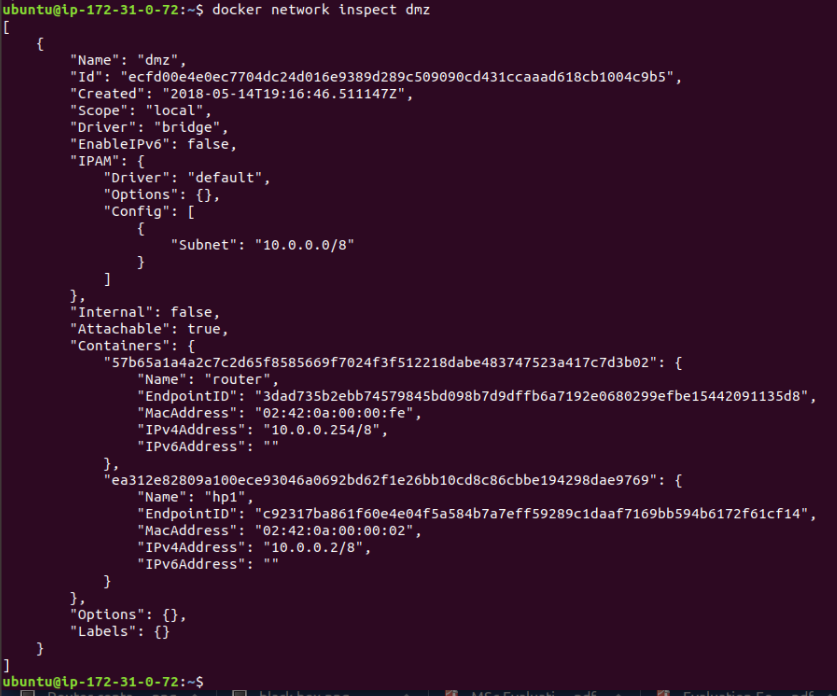
\includegraphics[width=160mm, scale=1]{Images/docker_network_inspect_dmz.PNG}
      \caption{Console Output of \textit{docker network inspect dmz}} 
      \medskip
      \small
		An image showing the console output obtained by executing the command \textit{docker network inspect dmz}. It can be observed that there are 2 containers on this network: The \textit{router} container, and the \textit{hp1} Cowrie container. 
\label{fig:docker-network-inspect-dmz}
\end{figure}


The correct routing of attack traffic from the \textit{router} container through the \textit{dmz} to the \textit{hp1} Cowrie container could be tested from inside the router container. Once inside the \textit{router} container, connecting over SSH or telnet to the \textit{hp1} honeypot and being presented with the Cowrie login prompt verifies the correct configuration of the network. Figure \ref{fig:cowrie-ssh-login-from-router} shows the console output when an SSH connection is attempted from the \textit{router} container to the \textit{hp1} container, demonstrating the correct routing of traffic within the \textit{dmz} network.

\begin{figure}[ht]
      \centering
      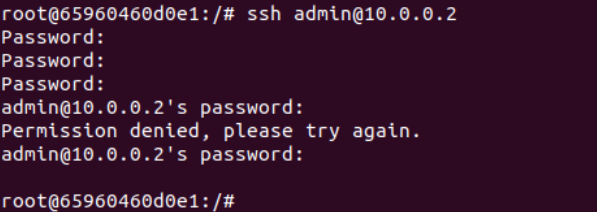
\includegraphics[width=160mm, scale=1]{Images/example-ssh-login-cowrie-container.PNG}
      \caption{A Denied SSH Login from the Router to a Cowrie Honeypot} 
      \medskip
      \small
		This screenshot shows a simulated attack session from the \textit{router }container to the \textit{hp1} Cowrie honeypot container. It can be observed that the ''attacker'' attempts to log in to  the \textit{hp1} container as user \textit{admin}. The first password provided for login is rejected, and a second prompt for the correct password is requested by the \textit{hp1} Cowrie honeypot. In this case, the attacker decides to cancel the login attempt rather than proceeding with a second login attempt.
\label{fig:cowrie-ssh-login-from-router}
\end{figure}

%\includewidefigure{cowrie-ssh-login-from-router}{A Denied SSH Login from the Router to a Cowrie Honeypot}{This screenshot shows a simulated attack session from the \textit{router }container to the \textit{hp1} Cowrie honeypot container. It can be observed that the ''attacker'' attempts to log in to  the \textit{hp1} container as user \textit{admin}. The first password provided for login is rejected, and a second prompt for the correct password is requested by the \textit{hp1} Cowrie honeypot. In this case, the attacker decides to cancel the login attempt rather than proceeding with a second login attempt.}{Images/example-ssh-login-cowrie-container.PNG}

    
%% 
%% SECTION 4: Visualisation
%%

\section{Visualisation of Attack Data} \label{LoggingAndVisualisationSection}
As decided in \textit{Section \ref{VisualisationDesignChoice}} as part of the design process, the data generated by honeypots in the Docker honeynet would be visualised using the ELK log processing stack on a separate EC2 server instance. The deployment of the EC2 management server instance was already described in \textit{Section \ref{DeployingTheManagementInstance}}, and this section details the installation and configuration of the tools on this instance to enable the processing and visualisation of the honeypot data.

\subsection{Management Server Instance}
The EC2 management server instance had already been deployed with sufficient hardware resources to meet the requirements of the ELK stack. Since the ELK stack is widely used for log processing and visualisation, there were plentiful resources available from which to learn, showing how to configure these open-source tools to work together.

Some complementary tools were also used in order to facilitate the use of the ELK stack for analysis of logs from a remote machine: In particular, Nginx and Filebeat. The configuration and interoperation of all of these tools is described in the following subsections.

	\subsubsection{Elasticsearch}
    Elasticsearch is an open-source search and analytics engine built on the Apache Lucene API. The fact that it supports analysis of JSON-formatted files made it an ideal choice for the analysis and indexing of the Cowrie logs, which are logged in JSON format.
    
    To set up the environment to run Elasticsearch, Java 8 was first required as a prerequisite installation. Once Java 8 has been installed, Elasticsearch was then also installed. Next, in order to configure Elasticsearch securely external access to the application needed to be restricted. This is important, since Elasticsearch provides a HTTP API that can be queried to perform manipulation on the data stored in the Elasticsearch index. If access to this was not restricted, the data in the index could be modified or removed without authorisation.
    
    By editing the \textit{/etc/elasticsearch/elasticsearch.yml} configuration file for Elasticsearch, external access was completely restricted by setting the access address \textit{network.host} to \textit{localhost}\footnote{The IP address 127.0.0.1 is known as the localhost address.}. This meant that Elasticsearch could only be accessed from the management instance itself on localhost, on the Elasticsearch default port 9200/TCP. 
    
	\subsubsection{Kibana}
    
    The Kibana visualisation engine was the second component of the ELK stack to be installed and configured. Kibana is an open-source analytics and visualisation platform, designed specifically to work with the Elasticsearch search platform. The use of Kibana in this project was intended to make analysis of the honeypot log files painless and immediate. 
    
    Kibana provides a web interface through which visualisations can be accessed. By configuring rules to visualise incoming log data, Kibana makes it possible to understand crucial information about the state of the system instantaneously.
    
    Similarly to Elasticsearch, it was important to set up Kibana to have restricted accessibility from external systems. In order to achieve this whilst still allowing an administrator to access the visualisations through the web interface, the Nginx reverse proxying tool was used.
    
		\subsubsection{Nginx}
        
Nginx is an open-source tool focused on providing services like web serving, reverse proxying, caching, and load balancing. \cite{Nginx} In this system, it was used to allow access to the Kibana web interface using reverse-proxying. 

An authentication step was configured with a single valid username-password credential to allow for authenticated login from a web browser. A small amount of additional configuration was then required to direct incoming HTTP traffic to the Kibana application\footnote{This involved the addition of the EC2 management server instance's public IP address to a Nginx  configuration file in the \textit{sites-available} directory.}.
      
	\subsubsection{Logstash}
    Logstash is an open-source log pipeline tool which accepts, processes, transforms and outputs data from log files provided to it, and was the final component configured on the management server instance. 
    
    As discussed in \textit{Section \ref{SecureLogTransfer}}, an SSL certificate was generated by using the private IP of the server in the SAN field. This would later be used by Logstash to verify the origin of log data shipped by Filebeat.
    
    %%Nice diagram: https://www.elastic.co/guide/en/logstash/2.4/advanced-pipeline.html
    In order to configure the processing components of Logstash, a number of configurations needed to be defined to deal with each of the incoming log formats: Input, filter and output configurations. These were all specified as part of the same file, \textit{03-cowrie.conf}. 
 \begin{itemize}
    \item \textbf{Input}
    
    Inputs are a field used to pass data into the Logstash pipeline. In this system, a single input was defined to accept data of type \textit{beats}, corresponding to data shipped by Filebeat. 

A port number was specified from which this data should be received by Filebeat. The path to the generated SSL certificate was also specified, so that the data received on this port could be verified by Logstash.
    \item \textbf{Filter}
    
    Filters are an intermediary processing step in the Logstash pipeline, where operations can be applied to the input data. An excellent tutorial was identified which explained a number of different filtering operations that could be applied to the Cowrie logs. These formed the basis of the filtering operations configured in this field\footnote{It should be noted that although substantial effort was expended to perform the similar filtering operations on the \textit{syslog} files generated by the router container honeypot, there were multiple compatibility issues encountered which resulted in the failure to visualise these logs on the Kibana web interface.}. \cite{FernandoDominiguezCowrieLogstashConfig}
    \item \textbf{Output}
    
    Outputs are last field in the Logstash processing pipeline, piping the results of the processing to a designated output process. In this case, the output process was Elasticsearch, which had been configured to listen for incoming data on localhost, port 9200. Some additional options were specified regarding the formatting of the data to be stored in the Elasticsearch index.
    \end{itemize}
    
    
\subsection{Honeypot Instance}
To provide the EC2 management instance with honeypot data to visualise, the logs generated by the honeypot containers on the EC2 honeypot instance needed to be aggregated and then transferred securely to the management instance. This was achieved as described below.

	\subsubsection{CRON \label{CRON}}
		
		A CRON job was configured to run every 60 seconds on the honeypot instance, shipping the honeypot logs from their respective container volumes to a defined location on the honeypot instance: The \textit{/var/logs/} directory. This meant that logs generated by all honeypots present would be aggregated in a single location on the honeypot instance.
        
\includecode{CRON Log Shipping Job}{This snippet shows 2 tasks scheduled using CRON, which copy the contents of the honeypot container volumes to the \textit{/var/logs} directory. These jobs are run every 60 seconds, the maximum possible frequency for a CRON job.}{Code_snippets/cron.txt}

	\subsubsection{Filebeat}
    Filebeat is an open-source application which was discussed in \textit{Section \ref{SecureLogTransfer}} in the context of securely transferring honeypot logs from the EC2 honeypot instance to the EC2 management instance using SSL certificates. The SSL certificate previously generated by the management server was shared with the honeypot instance using Secure Copy (SCP).
        
    The Filebeat configuration file, \textit{/etc/filebeat/filebeat.yml}, was configured to inspect the \textit{/var/log} directory on the EC2 honeypot instance for the presence of log files any time updated log files were added to it by CRON. It was then configured to send the logs to the EC2 management instance using private IP addressing, specifying the destination port to be the same as that configured in the \textit{input} field of the Logstash configuration file. Lastly, Filebeat was configured to use the SSL certificate generated by the EC2 management instance for all data transferred.


\section{Alert/Notification System}\label{AlertSystemSection}
As another important element of the cyber incident monitor identified in \textit{Section \ref{IncidentMonitoringDesign}}, the configuration of a threat notification system was the final step in the implementation of the cyber incident monitor.

\subsection{PSAD}
As explained in \textit{Section \ref{DesignChoicePSAD}}, PSAD was identified as the tool of choice to enable alerting of system administrators to potential attacks happening on the honeypot host. It was deployed on the honeypot instance in order to provide an instantaneous notification to system administrators of potential attacks. A basic configuration generated email alerts when probing of the honeypot instance was detected, sending notification emails to the address \textit{itsmyjobtofixtheproblem@outlook.com}, which could be specified in the \textit{/etc/psad/psad.conf} configuration file. It was possible to configure PSAD to check the state of the network event logs as frequently as desired, for which a reasonable frequency was chosen to be every 5 seconds.

\begin{figure}[ht]
      \centering
      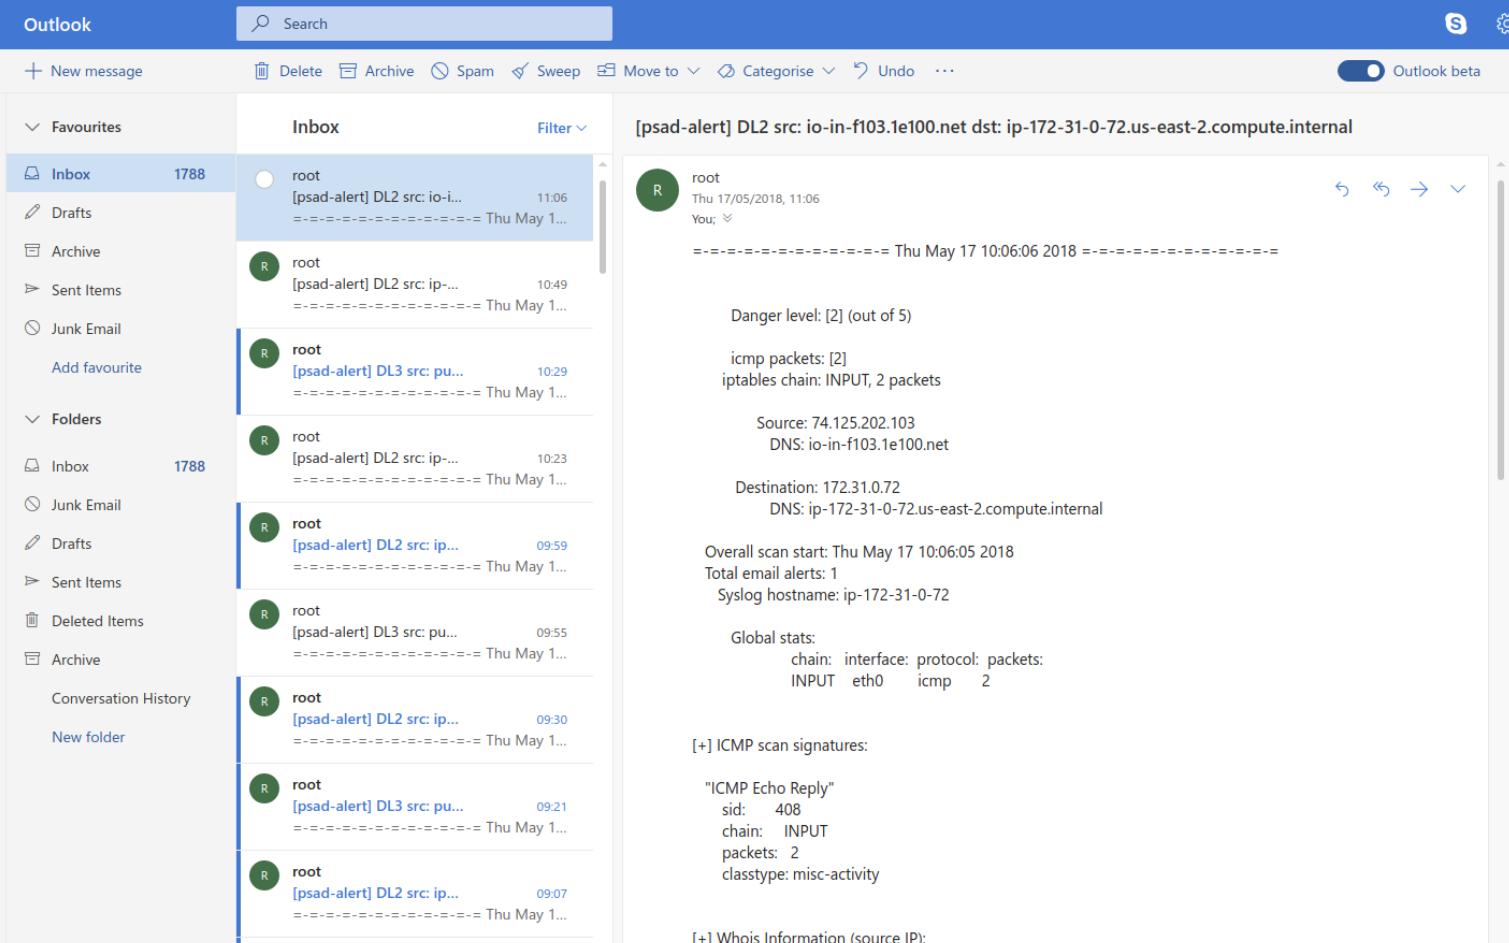
\includegraphics[width=160mm, scale=1]{Images/psad-email-alert.PNG}
      \caption{An Email Alert from PSAD} 
      \medskip
      \small
		This screenshot shows the email inbox to which PSAD was configured to send email alerts. It can be seen that a port scan generated an email alert shown in the right-hand pane of the email inbox. PSAD has detected that the source of the scan is a domain \textit{io-in-f103.1e100.net} which has sent a number of ICMP packets to the EC2 server instance, triggering this alert.
\label{fig:psad-email-alert}
\end{figure}

With PSAD it is also possible to completely blacklist or whitelist\footnote{Whitelisting an IP address means that it is added to a list of addresses that are considered trustworthy.} certain IP addresses by editing the \textit{/etc/psad/auto\_dl} configuration file. This functionality was used to reduce the number of false positives being generated by PSAD\footnote{After PSAD was initially configured, there were many email alerts generated from a particular server called \textit{chillipepper.canonical.com}. Upon contacting Canonical Ltd. about the possibility of their server being compromised and used to launch attacks, it was found that the alerts were being generated by benign Network Time Protocol (NTP) time synchronisation traffic.}.

\section{Summary \label{ImplementationSummary}}
By the time all of the system components had been configured and implemented as described in this chapter, an end-to-end system cyber incident monitoring system was in place.

\begin{itemize}
\item Attack sessions could be simulated, connecting to the EC2 honeypot instance over SSH or telnet and being presented with the router container login prompt. After authenticating with the router container, it was possible to connect in the same way to any container in the honeynet and interact with a Cowrie honeypot.
\item All activity generated from interactions with the Cowrie containers was being successfully shipped, processed and visualised, with the visualisation dashboard accessible from a web browser.
\item The entire Docker environment could be completely removed and redeployed with an identical configuration if required.
\end{itemize} 

Thus, the objective of developing a honeypot-driven cyber incident monitor had largely been achieved at this point, with much remaining scope for configuration of both the honeypots and the visualisations once attack data had been obtained. This system would be used to conduct a series of experiments focused on determining effective design for adaptive honeypots, detailed in \textit{Chapter 6}.